\documentclass[12pt, a4paper, twoside, titlepage]{report}

%
% File containing all the package declarations
%
\usepackage{./tex/mystyle}
\usepackage{./tex/abbreviations}

%----------------------------------------------------------------------------------------
%	DEFINITIONS
%----------------------------------------------------------------------------------------

\def \author {Katarzyna Sprawka}
\def \title {Numerical Assessment of Kidney Function from DCE-MRI}
\def \titlepl {Numeryczna ocena funkcjonowania nerek na podstawie obrazów DCE-MRI}
\def \supervisor {Prof. hab. dr inż. Andrzej Materka}
\def \auxiliarySupervisor {Dr inż. Marek Kociński}


%----------------------------------------------------------------------------------------
%	BODY
%----------------------------------------------------------------------------------------


\begin{document}

% Title page
% Strona tytułowa

\thispagestyle{empty}

\begin{center}
	\vspace*{-1.5cm}
	{\scshape\LARGE Lodz University of Technology} \\ 
	{\scshape\large Faculty of Electrical, Electronic,\\Computer and Control Engineering } \\
	{\scshape\large Institute of Electronics} \\
	
	\vspace{2.0cm}
	{\scshape\large Master of Engineering Thesis } \\
	
	\vspace{0.5cm}
	\textbf{\Large\title{}} \\
	
	\vspace{0.5cm}
	\textbf{\Large\author{}} \\
	
	\vspace{1.5cm}
	\textbf{\large Student's number: 213407}
	\vspace{4.25cm}
	
	\begin{flushright}
		\em \rm {\large Supervisor:} \\
		\textbf{\large \supervisor{}} \\
		\em \rm {\large Auxiliary supervisor:} \\
		\textbf{\large \auxiliarySupervisor{}}
	\end{flushright}
	
	\vfill
	{\large Łódź, 2018}
\end{center}

% Po drugiej stronie strony tytułowej pusta strona
\newpage
\thispagestyle{empty}
\mbox{}

% Abstract 
%
% Streszczenie
%
\newgeometry{left = 3cm, right = 2.5cm, top=2.3cm, bottom = 3cm}

\newpage	%░░░░░░░░░░░░░░░░░░░░▒▒▒▒▒▒▒▒▒▒▒▒▒▒▒▒▒▒▒▒░░░░░░░░░░░░░░░░░░░░
\thispagestyle{empty}
\pagenumbering{roman}
\setcounter{page}{1}

	\phantomsection \label{sec:Abstract}
	\addcontentsline{toc}{chapter}{Abstract}

	\begin{spacing}{1.0}
		\begin{center}
			%\vspace*{-3.35cm}
			{\scshape\normalsize Lodz University of Technology} \\ 
			{\scshape\normalsize Faculty Of Electrical, Electronic, Computer And Control Engineering} \\
			\vspace{0.5cm}	\textbf{\large\author{}} \\
			\vspace{0.3cm}
			{\scshape\footnotesize Master of Engineering Thesis} \\
			\vspace{0.25cm}
			\textbf{\large\title{}} \\
			\vspace{0.25cm}
			{Łódź, 2018~r.}
		\end{center}
		
		\begin{flushleft}
			{\supervisor{}}\\
			{\auxiliarySupervisor{}}\\
		\end{flushleft}

		
		\begin{center}
			{\bf\large Abstract}
		\end{center}
	\end{spacing}
	
	\begin{spacing}{1.0}
		\begin{small}

The kidneys maintain whole body homeostasis enabling the organism to function in an optimal environment. The metrics of the renal function is glomerular filtration rate (GFR) and its monitoring is essential for prognosis, diagnosis and treatment of renal diseases. Clinically used chemical methods are cumbersome and do not allow for single kidney GFR (SKGFR) estimation,  in contrary to the analysis of the dynamic contrast enhanced magnetic resonance imaging  (DCE-MRI), which enables a non-invasive examination of both renal function and structure in a single imaging session. However, there is a lack of methods enabling reliable renal function quantification without human interference.

The works included in this thesis are a part of the project, which aims to develop entirely data-driven method of GFR estimation directly from DCE-MRI---fast, efficient and accurate enough to be used in clinical practice. 
The scope of this thesis was to develop an library for quantitative analysis of DCE-MRI in Python programming language to be used in the target method and to compare the performance of different pharmacokinetic (PK) models in renal function assessment applications.

First, the labels of both kidneys and aorta were depicted on registered DCE-MRI sequences. In order to remove the region of the renal pelvis, the kidney voxel-wise segmentation on the basis of intensity time courses was performed with the use of principal component analysis (PCA) and k-means clustering algorithm. Average contrast agent concentration-time curves of the functional region of each kidney were then fitted to the four PK models: \textit{Tofts and Kermode} (TK), \textit{extended Tofts and Kermode} (ETK), \textit{Patlak-Rutland} (PR) and \textit{two-compartment exchange} (2CXM) models. From the obtained model parameters, the SKGFR and total GFR were calculated.   

The developed method was tested on DCE-MRI sequences of ten healthy subjects. Obtained total GFR values were compared with the values obtained in iohexol-GFR and serum creatinine tests.
The results showed that 2CXM is the most accurate and precise of tested PK models with reference to the iohexol-GFR and its performance is comparable with a serum-creatinine test. 

The conclusion was drawn that 2CXM can be used in a final step of the GFR estimation in the target method and the developed library enables its implementation.   

		
		
		\end{small}

		
		\vfill
		\normalsize \noindent \textbf{Keywords:} DCE-MRI, kidney, glomerular filtration rate, pharmacokinetic modelling, quantitative analysis, kidney segmentation.  
				
				\end{spacing}	

	\newpage
\thispagestyle{empty}
\mbox{}	

	

% Acknowledgements
\chapter*{Acknowledgements}

\thispagestyle{empty}

\phantomsection \label{sec:acknowledgements}
	\addcontentsline{toc}{chapter}{Acknowledgement}
	
First and foremost, I would like to express my sincere gratitude to Professor of the University of Bergen, Arvid Lundervold, for his enlightening guidance throughout this project and warm hosting me during the stay in Norway, for his encouragement and enthusiastic approach, immense knowledge, and most importantly for inspiring me with the world of medical imaging.

I also would like to thank my supervisors from my mother university, Professor Andrzej Materka and PhD.~Marek Kociński for the useful comments and remarks both the substantive and editorial ones, which helped to give this dissertation its final shape. Without their assistance this thesis would have never been accomplished.

\newpage
\thispagestyle{empty}
\mbox{}	
	

% Abbriviations
%\chapter*{List of Abbreviations}
%

\fancypagestyle{plain}{
	\fancyhead[LE,RO,RE,LO]{}
	\fancyfoot[]{}
	\renewcommand{\headrulewidth}{0pt}
}

\thispagestyle{empty}
%\pagenumbering{gobble}
%%
%\phantomsection \label{sec:Abbreviations}
	%\addcontentsline{toc}{chapter}{List of Abbreviations}


\thispagestyle{empty}
\glsaddall
\thispagestyle{empty}
\printglossary[ nogroupskip, style=super, type=\acronymtype, nonumberlist]
%
\thispagestyle{empty}

%\newpage
\thispagestyle{empty}
%\mbox{}

%, 

\fancypagestyle{plain}{
	\fancyhead[LE,RO,RE,LO]{}
	\fancyfoot[C]{\thepage}
	\renewcommand{\headrulewidth}{0pt}
}


% Content 
\phantomsection \label{sec:content}
\addcontentsline{toc}{chapter}{Contents}
	\begin{spacing}{1.1}
		\tableofcontents
	\end{spacing}
%\newpage



%Introduction

\pagenumbering{arabic}
	\setcounter{page}{1}
	
%\fancyhead[LE,RO]{{\small{\author}}\linebreak{\small\textsl{\title}}}
%\fancyhead[RE,LO]{}
%\renewcommand{\headrulewidth}{1pt}
	
\chapter{Introduction}
	%\addcontentsline{toc}{chapter}{Introduction}

%To be done


\lettrine[lines=3, slope=1em, findent=-0.8em]{A}{ccording to the beliefs of ancient Hebrews}, the kidneys are the seat of the human soul and consciousness. They were also assosiated with the felling of the fear and sadness \cite {maio1999metaphorical}. Today, more mundane, but not less important tasks are being assigned to them. 

Kidneys, although often underestimated, are the fundamental organs of human body and their working mechanism is extremely complex. Their essential task is to remove wastes from the organism but their functionality is much wider. They are also involved in maintaining acid-based balance, regulating the blood pressure and are major endocrine organs, which secret three important hormones: \textit{erythropoietin}, \textit{calcitriol} and \textit{renin} \cite{saladin}. In short terms, they maintain whole body homoeostasis, which is essential for overall health of the organism. 

Gradually progressing loss of kidney function known as a chronic kidney desease is a~ growing world-wide problem. As much as 8--16\% of whole population suffers from this condition \cite{statistics}. It significantly decreases comfort of life and in extreme cases leads to death. What is more, it was shown that renal diseases are risk factor for development of cardiovascular diseases \cite{cardiovascular_diseases}.
Because of the fact that symptoms do not resemble renal failure, approximately 90\% of the ill are unconscious of it until late stages \cite{national_kidney_foundation}. That is why there is the demand for methods, which enable fast and accurate measurement of renal function required for all of three: prevention, monitoring and therapy.

The metrics of the level of kidney function is \textit{glomelural filtration rate} (GFR) \cite{traynor2006measure}. Good performance of the several important functions of the kidney are dependent on the GFR value. Not only does it allow for assessment how well our kidneys are working, but also it can determine the stage of kidney disease.
The gold standard of GFR measurement incorporates injection of the exogenous marker that is freely filtered by the kidney, and that does not undergo metabolism, tubular secretion or absorption. An example of such a~marker can be insulin.
However, in clinical practice usually the endogenous marker is used such a creatinine or urea and GFR is estimated applying robust algoritms \cite{delanaye2012measuring}.
Although chemical methods allow for accurate GFR estimation, they are not very practical in clinical use. Not only are they time-consuming and expensive but also they can be cumbersome. What is more they provide information about combined GFR value and cannot be used for a single kidney function assessment. Thus, other methods are desired \cite{bokacheva2008assessment}.

An innovative approach in estimating renal function is performing dynamic contrast-enhanced magnetic resonance (DCE-MRI), which provides time-varying images of the abdominal.
The analysis of the obtained time-intensity changes as a function of time provides important information about renal performance \cite{bokacheva2008assessment, khalifa2014models}. Traditionally, this evaluation is performed by experienced observer, although this method is very subjective and strongly depends on the experience of the expert. Other technique involves fitting tissue intensity changes to \textit{pharmacokinetic} (PK) models, which allows quantification of renal function \cite{khalifa2014models}. Even though this strategy is gaining more and more supporters, most of the methods still require interference of the human at some stage, which makes them vulnerable to human factors. 

\section{Aims and scope of the thesis}
The works included in this thesis are the part of the bigger project realised at the University of Bergen in Norway, which aims to develop entirely data-driven method of GFR estimation directly from DCE-MRI, which would be fast and efficient and accurate enough to be used it clinical applications.  
 
The overarching aims of this thesis is to create the library for GFR estimation by pharmacokinetic modelling in Python programming language and to compare the performance of different PK models in renal function estimation. What is more, it should be decided if any of them is accurate enough to be used in the target method of fast GFR estimation. 

The structure of this thesis is as follows:
because of the fact that the thesis is connected with the assessment of the renal function Chapter 2 deals with the basics of the renal anatomy and physiology in order to understand the mechanism of glomerural filtration and importance of the metric, which is GFR.
Chapter 3 focuses on the basic principles of operation of DCE-MRI and introduces the current trends and obstacles in its examination.  
Furthermore, Chapter 4 is devoted to the issue of quantitative analysis of DCE-MRI. 
It discusses the  basics of tracer kinetic theory and lists all components required for pharmacokinetic modelling.  
Next, Chapter 5 and Chapter 6 focus on the practical part of the work.  
Chapter 5 describes in details the subsequent steps of DCE-MRI processing, whereas Chapter 6 presents obtained results. 
Finally, in Chapter 7, the obtained results are discussed and the comparison of different PK models is covered. 




% Chapter 1-Aims and scope of the project
\chapter{Aims and scope of the work}

% Chapter - The kidney
\chapter{The blood filter}
	
There is no life without metabolizing, and metabolism always produces variety of waste products, which accumulated in the tissues are toxic to the organism. Some of them are removed from the body by respiratory tracts, others through digestive system and some of them are extracted through the sweat glands. However, there is no doubt that the urinary system plays the major role in waste extraction \cite{saladin, health_and_disease}.

The main organs of the urinary system are the kidneys. It is them, which perform the filtering function. The remaining ones,  ureters, urinary bladder, and urethra, form the urinary tracts and are responsible only for transforming and storing the urine \cite{saladin}. In this chapter the anatomy and physiology of the kidneys will be briefly introduced.

\section{Structure of the kidney} 

The kidneys are  bean-shaped, usually paired structures located at the back of the abdominal cavity in the retroperitoneal space. They lie on at the level of vertebrae T12 to L3.
The right kidney is slightly lower than the left one, because of the close proximity to the the liver \cite{saladin, health_and_disease}. 

The average healthy adult kidney weights around 150\,g, is 11\,cm long, 6\,cm wide and 3\,cm thick \cite{kidney_dimensions, saladin}. As mentioned before, humans usually have two kidneys, however not always.  Some people are born with only one of them.  In such case, the present kidney is as heavy and big as the two kidneys together would be. In most cases it doesn't affect normal live \cite{onekidney}. 

The kidneys are surrounded and protected by three types of connective tissue, from the outter part: 
\begin{inparaenum}[(1\upshape)]
\item \textit{renal fascia} anchoring the kidneys and the neighbouring organs to the abdominal wall;
\item \textit{adipose capsule}, which is a layer of fat tissue holding the kidney in place;
\item \textit{renal capsule}, made of fibrous tissue, firmly enclosing the organ and protecting it from traumas and infections \cite{saladin, health_and_disease}.
\end{inparaenum} In the medial concave surface, there is a~slit called \textit{hillum}, which is the place where the  renal  artery enters and the renal vein and the ureter leave the kidney. The hillum extens into the \textit{renal sinus}, which is a large cavity occupied by blood and lymphatic vessels, nerves, urine-collecting structures and adipose tissue \cite{health_and_disease}.

The renal parenchyma is divided into two major parts: 
\begin{inparaenum}[(1\upshape)]
\item the outer 1\,cm thick portion of the kidney,  \textit{renal cortex}
\item the inner \textit{renal medulla}
 \cite{saladin, health_and_disease}.
\end{inparaenum}
The cortex projects into the kidney forming \textit{renal columns}, which divide the medulla into 10-14 \textit{renal pyramids}. Each of them has a characteristic shape of a cone with the wide base facing the cortex and the tip attached to the sinus called \textit{renal papilla}.  The papilla of each pyramid points towards the \textit{minor calyx} collecting its urine. Few of them converge into the \textit{major calyx}, whereas the all latter ones form the funnel-shaped basin, the \textit{renal pelvis}, which is the extension of the \textit{ureter} transforming the urine to the bladder \cite{saladin, health_and_disease, mosby}. The gross anatomy of the kidney is illustrated in Figure~\ref{fig:kidney_anatomy}.

	%\vspace*{-1.5cm}
\begin{figure}[H]
		\centering
		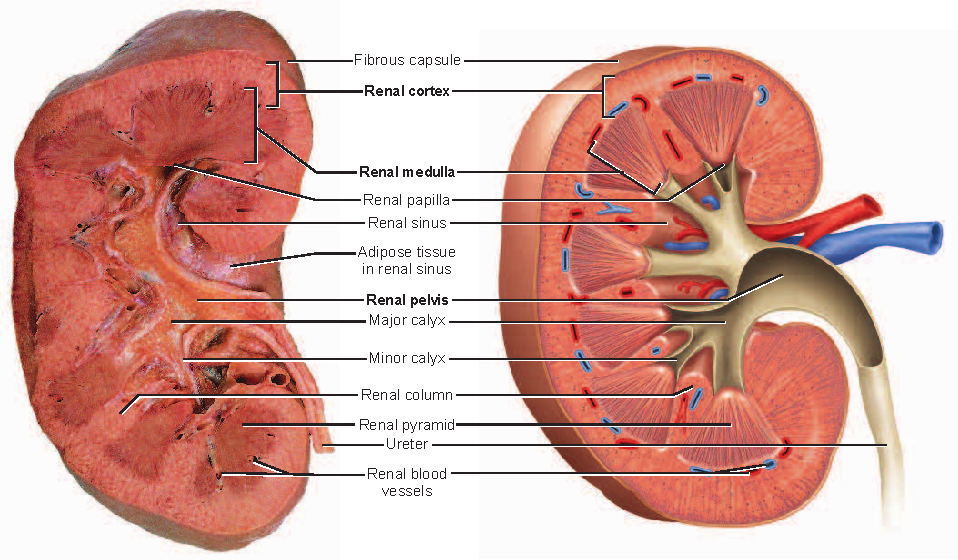
\includegraphics [height = 8cm]{kidney}
		\caption [Gross kidney anatomy]{Gross anatomy of the kidney \cite{saladin}}
		\label{fig:kidney_anatomy}
	\end{figure}
\subsection{The nephron} 

As it is with most of the aspects of the human anatomy, the most interesting features of the kidney are invisible with naked-eye. 
The basic microscopic functional units of the kidney are nephrones. Above million of them enables the kidney to perform its functions \cite{health_and_disease}. Each of them is a tiny coiled tube, called the \textit{renal tubule}, with a bulb at the end, the \textit{renal corpuscle}, and extends through both the cortex and the medulla \cite{saladin}.

The renal corpuscle is composed of the two-layered \textit{glomerular (Bowman) capsule} enclosing the
\textit{glomelurus}, which is a cluster of capillaries. The renal tubule is a~duct leading from the glomelural capsule to the pyramid papilla. It can be divided into several regions, subsequently from the glomerular corpuscle: 
\begin{inparaenum}[(1\upshape)]
\item the \textit{proximal convoluted tubule} (PCT);
\item the \textit{nephron loop (loop of Henle)}, which consists of the \textit{descending and ascending limbs};
\item the \textit{distal convoluted tubule }(DCT);
\item the \textit{collecting duct} receiving the fluids from the DCTs of few nephrons. Multiple of them merge and form papillary ducts, which lead  to the minor calyx.
% \cite{saladin, health_and_disease}.
\end{inparaenum}
Each of the segment has a distint cellular appearance and function \cite{saladin, health_and_disease, mosby}.

Every functional unit of the kidney is supplied with the blood by a small blood vessel called the \textit{afferent arteriole}, whereas the \textit{efferent  arteriole} takes it back. The blood leaving the nephron, flows  into  a
network of \textit{peritubular  capillaries} surrounding the renal tubule \cite{saladin, health_and_disease} The particular parts of the nephron are depicted in Figure~\ref{fig:nephron}.

\begin{figure}
		\centering
		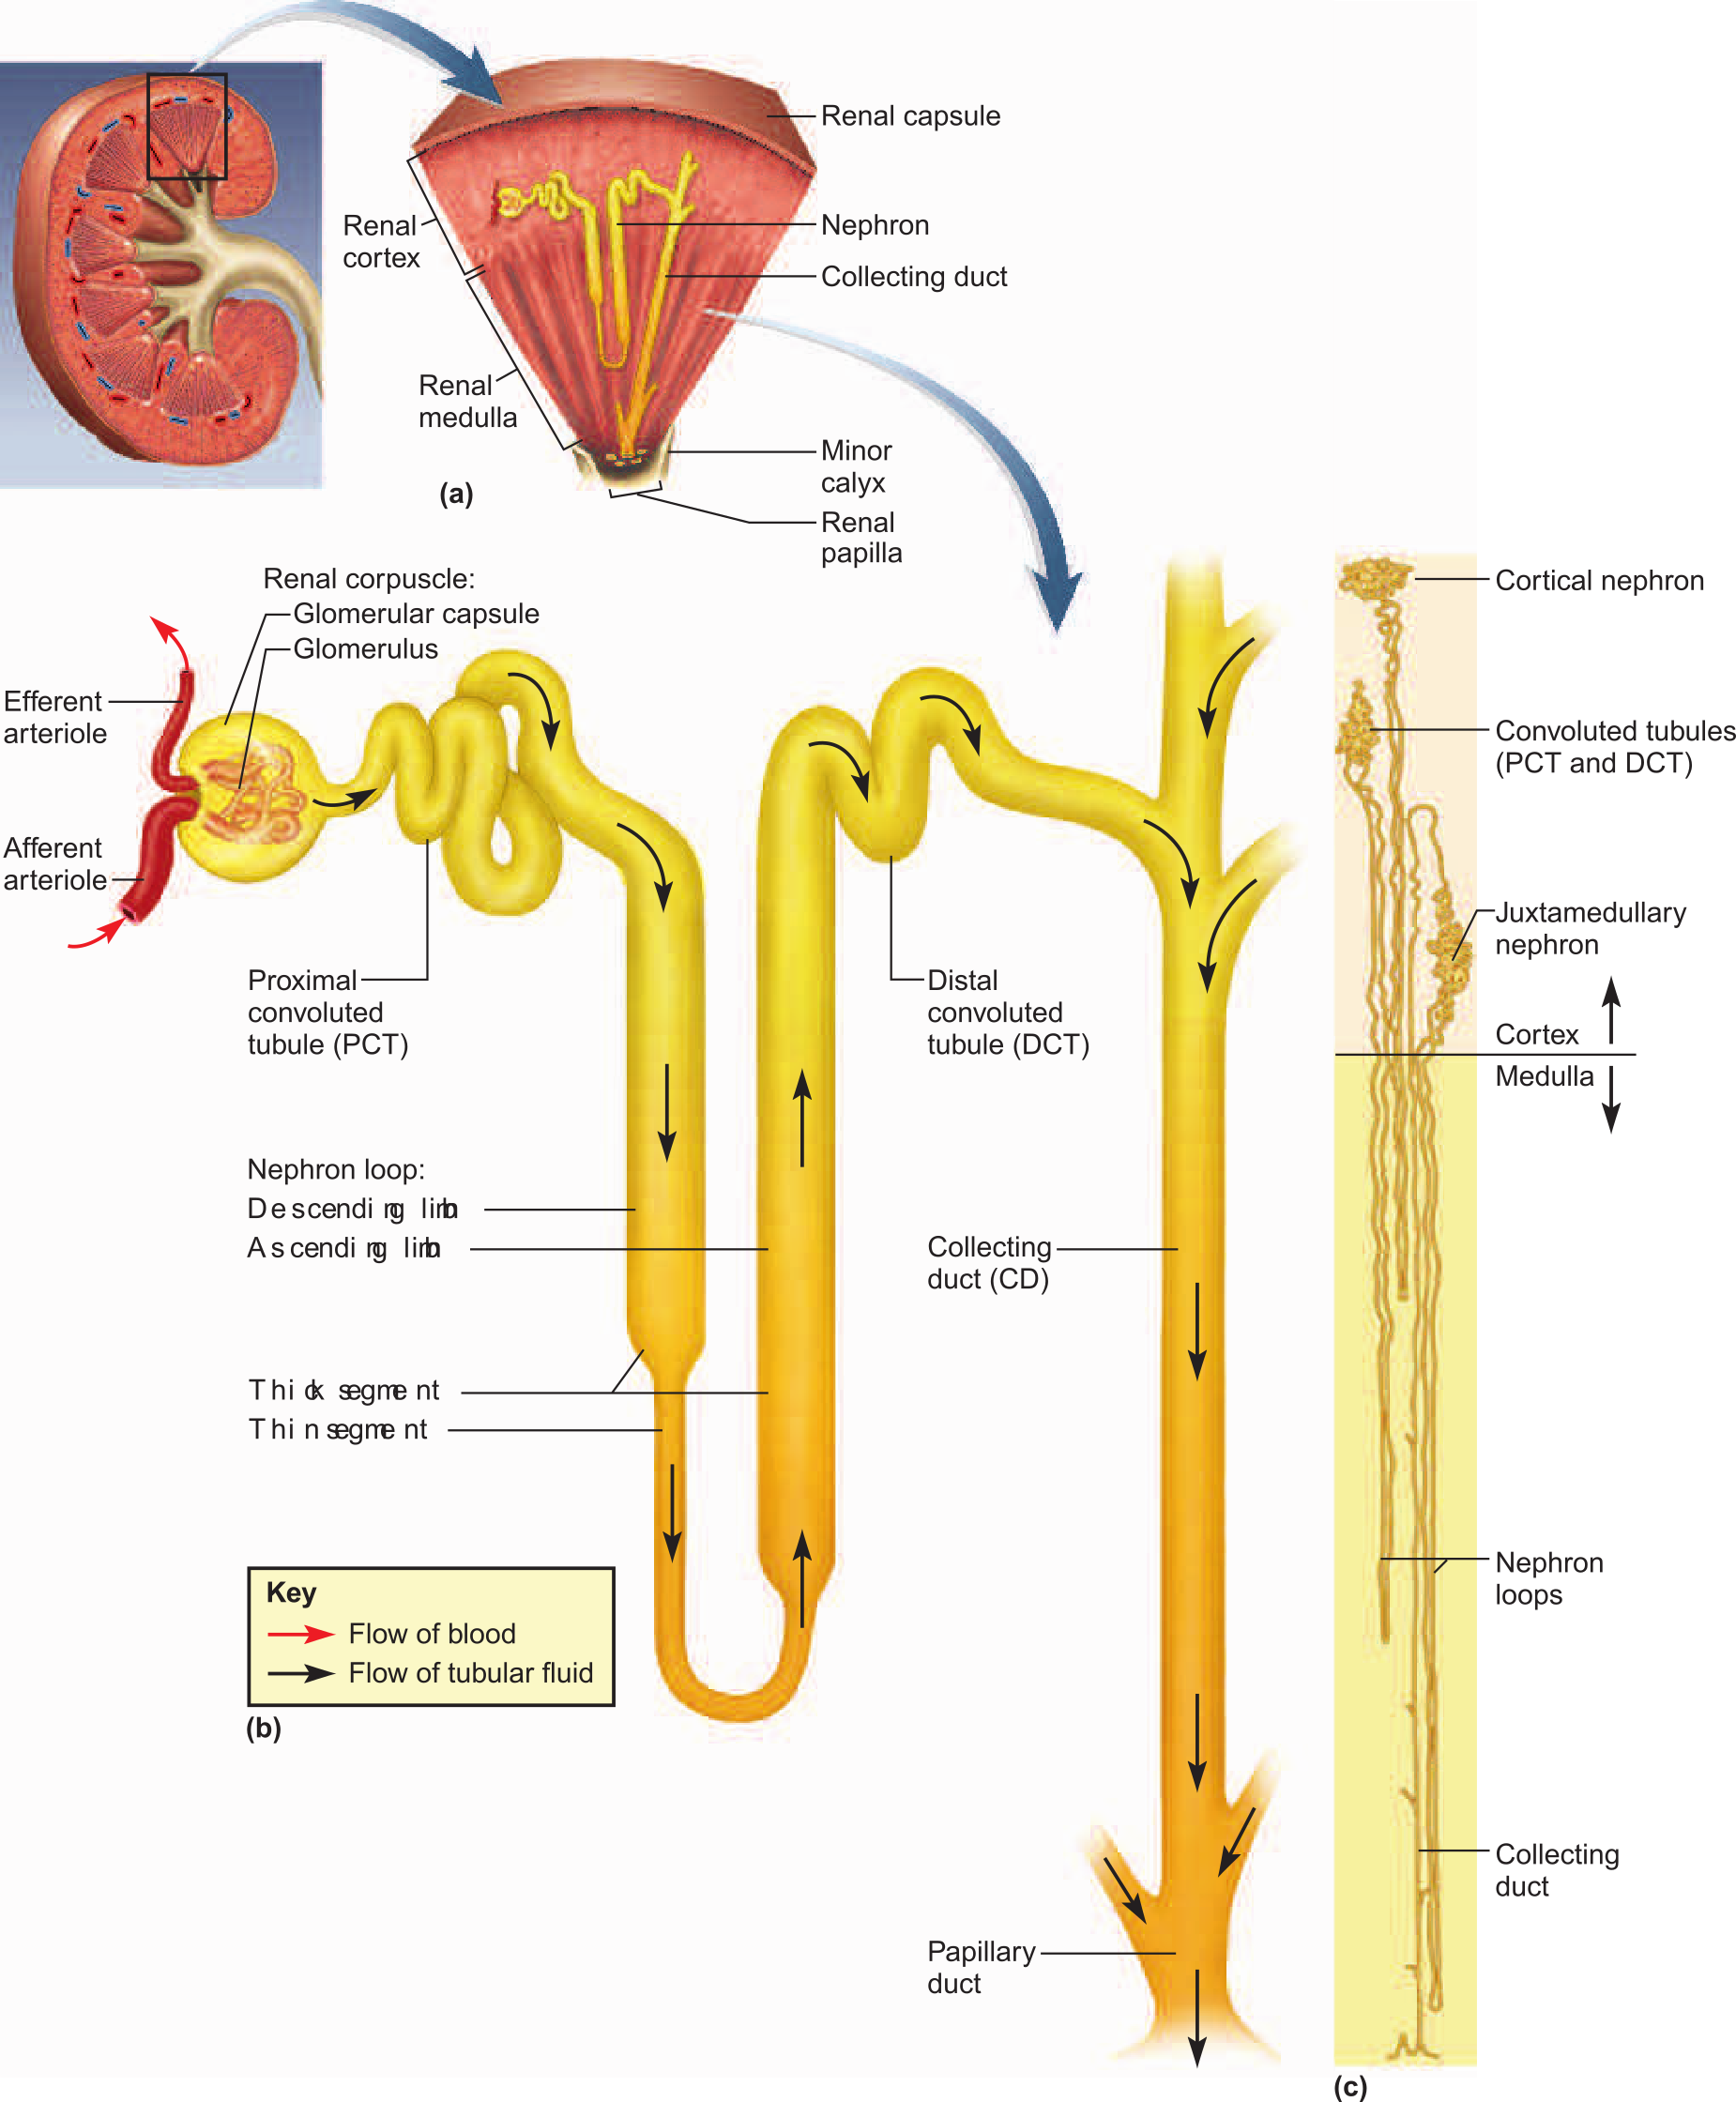
\includegraphics [height = 20cm]{nephron}
		\caption [The structure of the nephron]{The structure of the nephron \cite{saladin}}
		\label{fig:nephron}
	\end{figure}



\section{Functions of the kidney} 

Despite the fact that the key function of the kidneys is purifying the blood, the other ones are equally important. Kidneys are responsible for maintaining the homeostasis of the whole body due to which, all organs can work in an optimal environment.
It is crucial for a proper functioning of whole organism \cite{mosby}. One can conclude that the role of kidneys is enormously important. Indeed, the kidneys are involved in the following processes:
\begin{description}
		%\renewcommand\labelitemi{$\blacksquare$}
		\item [Blood filtering.] The kidneys filter the blood from metabolic waste, excessive amounts of salts, toxins and then excrete unwanted substances in the urine \cite{saladin, health_and_disease, mosby}.
		
		\item [Osmoregulation.]	For a proper functioning of the organism, the concentration of the salts in the body has to remain relatively the same. The kidneys influence this concentration by controlling the amount of water and solutes excrected from the organism \cite{sturkie1986kidneys}.	
		
		\item [Maintainance of water balance.] The kidneys control the amount of water conserved and eliminated in the urine so that the amount of body water remains on the stable level \cite{jequier2010water}.
					
		\item [Blood pressure regulation.] Maintaining the normal blood pressure is achieved in two ways: \begin{inparaenum}[(1\upshape)]\item if the blood pressure drops, the kidneys release the enzyme \textit{renin}, which activates the blood protein \textit{angiotensin}, making the blood vessels to constrict. What is more, angiotensin triggers the mechanism which increases the absorption of water and sodium, which in turn increase the blood volume; \item by regulating the amount of water, which was mentioned before \cite{guyton1972arterial}. \end{inparaenum} 
			
		\item [Maintainance of the acid-base balance.] The food contained in our diet can acidify or alkalize the organism. If the pH level is out of the tolerable boundaries, enzymes and proteins break down, which in extreme cases can lead to death. Kidneys in collaboration with the lungs are responsible for maintaining healthy pH of the body fluids. While the lungs' task is to regulate carbon dioxide ($CO_{2}$) concentration, the kidney acts by reabsorbing or regenerating bicarbonate ($HCO_{3}^{-}$) from the urine and excreting hydrogen ions and fixed acids into the urine \cite{hamm2015acid}.
	
	\item [Red blood cell production.] If the level of oxygen in the tissues is insufficient, the kidneys release \textit{erythroprotein}, the hormon stimulating the bone narrow to red blood cells production \cite{donnelly2001erythropoietin}. 

\item [Keeping the bones strong.] The kidneys, together with the liver, synthesize the active form of vitamin D called \textit{calcitriol} (1,25-dihydroxycholecalciferol) enabling the body to absorb calcium and phosphorus, which are the crucial minerals for strengthening the bones \cite{williams2009vitamin}.

\item [Prevent the hunger.] In the situation of extreme starvation, the kidneys can synthesize glucose from non-carbohydrate carbon substrates, breaking down other molecules. This phenomena is known as \textit{gluconeogenesis} \cite{newsholme1967control}.
%\item [Hormones degradation.] The kidneys take part in degradation of hormones such as \textit{parathyroid hormone} or \textit{insulin} \cite{emmanouel1980role}. 
%					
	\end{description} 

\subsection{Urine formation} 
Everyday, our kidney filter as much as 200 litres of fluid which is 60 times volume of blood in the body, and excrete 1.5 litres of urine \cite{saladin}. These enormous amounts are a~result of complex process involving numerous exchanges between a nephron and the blood stream. The process of the urine formation can be divided into 4 stages:
\begin{enumerate}
\item{\textbf{Glomerular filtration.}} When the blood enters the glomerulus through the afferent arteriole, the first step begins. Sievelike walls of the glomerular capillaries  pass every molecule smaller than 3\,nm to the glomerulal capsule. These molecules include the water and some solutes as glucose, electrolytes, fatty acids, nitrogenous wastes, amino acids and vitamins. On the other hand, they are impermeable to the larger components such as protein molecules and blood cells.  The diameter of the afferent arteriole is larger than that of efferent one, which gives the capillaries a large inlet and a small outlet. This in turn causes the pressure in the glomerulus to be much higher than elsewhere in the organism. Because the high pressure overrides the reabsorption, the movement of the particles occurs. This movement  of  the components, from  the  blood  into  the Bowman's capsule is known as \textit{glomerural filtration} and the fluid in the glomerular capsule, \textit{glomerular filtrate} \cite{saladin, health_and_disease}.

  
\item{\textbf{Tubular reabsorption.}} The filtrate passing through the renal tubule apart from wastes, contains  also water and many other useful substances such as ions and nutrients, which is a huge loss to the organism. Thus, they are being regained and returned to the bloodstream during the \textit{tubular reabsorption}. The movement is not direct but involves also extracellular fluids and is obtained through the \textit{diffusion}, \textit{osmosis} and \textit{active transport} \cite{health_and_disease}.
 
\item{\textbf{Tubular secretion.}} At this stage the final adjustment of the content of the urine is made. Wastes, toxins and unnecessary substances are passed from the blood to the renal tubule. What is of great importance, in this process also the hydrogen and bicarbonate ions can be removed in order to regulate the acid-base balance of the body \cite{health_and_disease}.

\item{\textbf{Urine condensation.}} When the filtrate enters the collecting duct, it becomes the urine. In order to prevent the water loss and keep the fluid balance of the body, during the last step, the water is returned to the tissue fluid and the bloodstream, which makes the urine more and more concentrated \cite{saladin}.

\end{enumerate}
Urine formulated in such a way is then extracted from the organism. The above stages are summarized in Figure \ref{fig:urine}.
\begin{figure}[H]
		\centering
		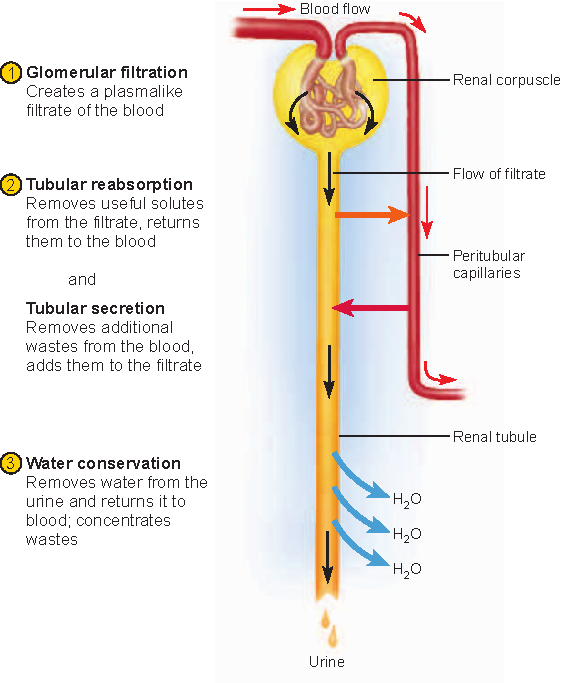
\includegraphics [width = 9.5cm]{urine}
		\caption [Process of the urine formation]{Process of the urine formation \cite{saladin}}
		\label{fig:urine}
	\end{figure}

\subsection{Glomerular filtration rate}
\textit{Glomerural filtration rate} (GFR) is a volume of fluid filtered during glomelural filtartion from the renal glomerular capillaries into the Bowman’s capsule per unit time by two kidneys combined and its unit is mL/min \cite{gfr_dictionary}. After standardisation, which is recalculation for standard \textit{body surface area} (BSA), GFR is expressed in mL/min/1.73\,m\textsuperscript{2} \cite{saladin}. 

The GFR in healthy adult kidneys is equal approximately 90--130\,mL/min/1.73\,m\textsuperscript{2} \cite{normal_values}. Lower at birth, it approaches its adult value at the age two and maintains its level till the age of fourty, when it starts decreasing again \cite{weinstein2010aging}. 
Appropriate GFR determines performance of several basic functions of the kidney. Neither too low, nor too high GFR is healthy to the organism \cite{saladin}.

In clinical practice, GFR is an approximate estimator  of the number of active nephrons and is concidered as a unit of level of kidney function. What is of great importance, GFR can also determine the stage of chronic kidney disease   \cite{traynor2006measure}.
GFR between 60--120\,mL/min/1.73\,m\textsuperscript{2} is considered normal, healthy value,%, although value under 90 should already be a reason of special attention, because it may mean early stages of renal malfunction.
below 60\,mL/min/1.73\,m\textsuperscript{2} indicates definite kidney desease, while the number under 15\,mL/min/1.73\,m\textsuperscript{2} is associated with renal failure \cite{national_kidney_foundation_values}. The reference values of GFR are shown in Figure \ref{fig:gfr}.  



\begin{figure}[H]
		\centering
		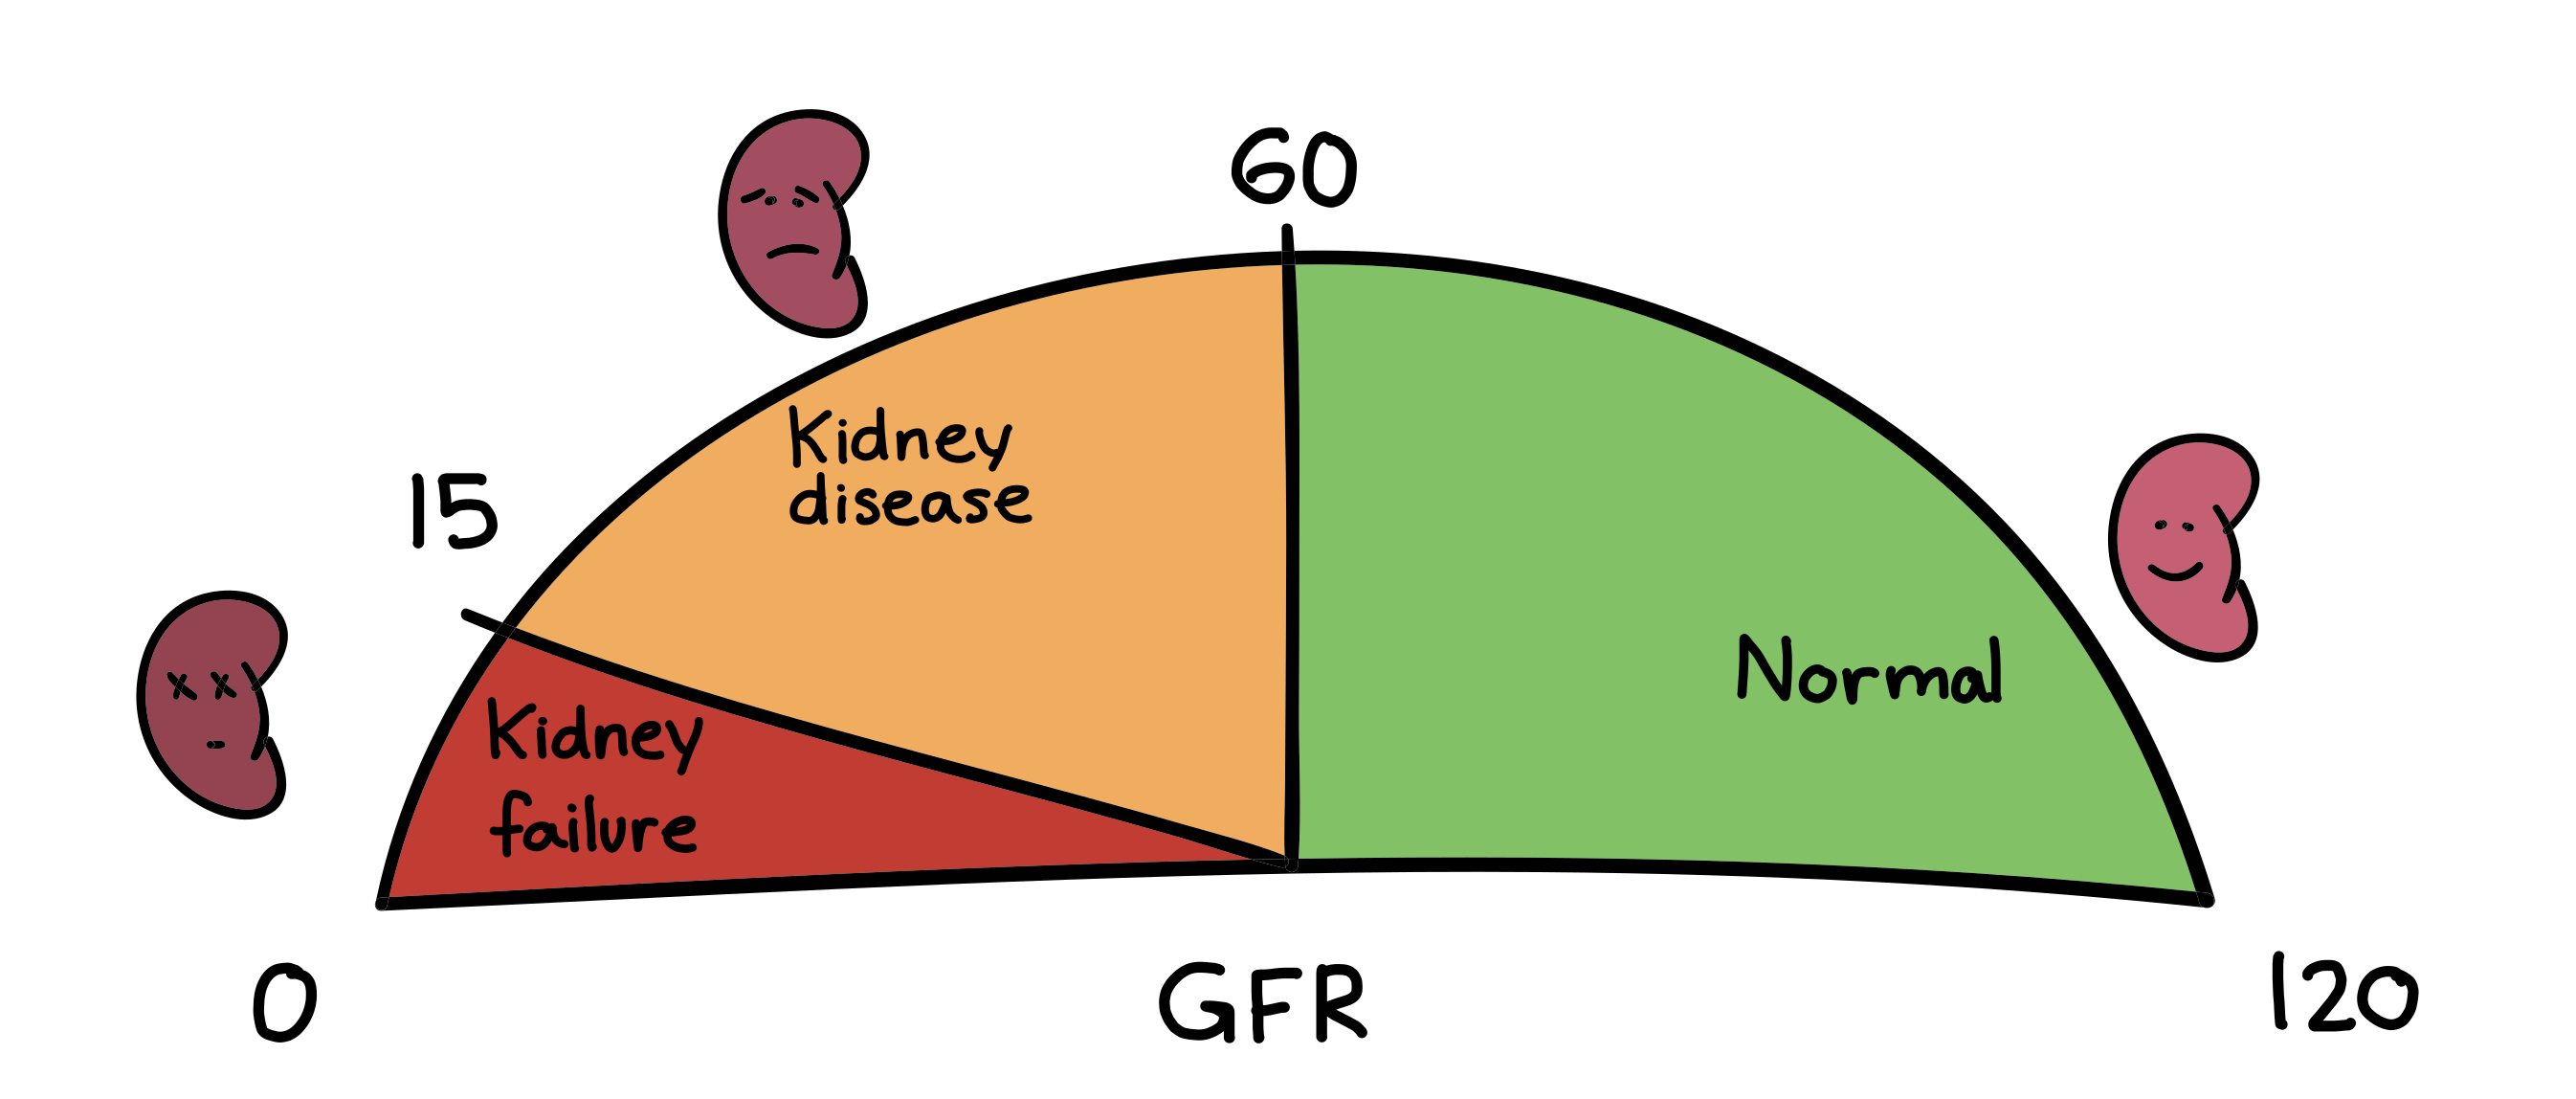
\includegraphics [width =12cm]{gfr_values}
		\caption [GFR reference values]{GFR reference values \cite{referencevalues}}
		\label{fig:gfr}
	\end{figure}

Due to the fact that the concentration of the particular substance in the blood and the urine is influenced not only by glomerular filtration, but also by tubular reabsorption and secretion, GFR cannot be measured directly by comparing the urine and blood concentrations. In such a way one would rather obtain \textit{renal clearance}, which is a volume of blood plasma from which a particular waste is completely removed in a~unit time \cite{saladin} This dependency is expressed as follows:
\begin{equation}
\begin{aligned}
&glomerular\;filtartion\;of\;the\;waste\\
-\quad&tubular\;reabsorption\;of\;the\;waste\\
+\quad&tubular\;secretion\;of\;the\;waste\\
\midrule
&renal\;clereance
\end{aligned}	
\label{eq:gfr_formula}
\end{equation}
For that reason, GFR measurement requires a~substance that is neither secreted nor reabsorbed by the nephrons, which implies that its entire amount in the urine is passed there by glomerular filtration. Unfortunately, there is no single solute appearing in urine and naturally produced by the body, which doesn't undergo the tubular secretion or reabsorbtion to some degree \cite{delanaye2012measuring}. 

However, in the nature there appear a substance whitch accomplishes the above conditions, namely insulin. One method of accurate measurement of glomelural filtration rate incorporates injecting insulin and subsequently measuring the rate of urine output and the concentrations of inulin in the blood and urine. For insulin, the GFR is equal to the renal clearance \cite{saladin, delanaye2012measuring}.


Even though this method is considered the gold standard in the GFR measurement, due to its limitations it is not a clinical routine if very accurate measurements are not required. This special cases include transplant donors or scientific research \cite{traynor2006measure}. 
Other, more frequently used techniques involve using endogenous markers such a \textit{creatinine} and estimating GFR by applying validated algoritms \cite{delanaye2012measuring}. 
%This method is usually accurate enough to be used in clinical practice.
 

% Chapter - DCE-MRI
\chapter{Dynamic Contrast Enhanced MRI}
	
Medical Imaging started with the development of X-rays by Wilhelm Röntgen in 1895, for which he received a Nobel Price \cite{rontgen1896new}. 
An enormous progress has been done since that time and numerous different imaging methods were developed, which found various applications in a medical field. Possibility of creating  visual representations of human interior as well as tissues and organs processes thus functionality much facilitated medical diagnosis and prognosis.   
Some imaging techniques has became an integral part of clinical care (i.e Computer Tomography, Magnetic Resonance Imaging, Positron Emission Tomography), whereas there exist one, which still needs to prove its utility. 

In this chapter the imaging technique, which is DCE-MRI will be introduced and its mechanism of imaging will be presented.

\section{Fundamentals of MRI}
In order to understand the mechanism of acquiring DCE-MRI sequences, it is inevitable to introduce the principle of operation of \textit{Magnetic Resonance Imaging}~(MRI).

MRI is an imaging technique based on the phenomena of induced nuclear  magnetism in the patient. Every molecule possessing a nuclei with an odd number of protons or neutrons  have a spin, implying a weak though observable randomly oriented nuclear magnetic moment. 
This particles include for example \textsuperscript{1}H, \textsuperscript{13}C, \textsuperscript{31}P, \textsuperscript{23}Na, \textsuperscript{19}F \nocite{bronzino1999biomedical}\cite{biomedical_hanbook_imaging}. If placed in a strong static magnetic field, these moments strongly tend to align parallel to the external field. Some of them will align antiparallel to the field, however there will always be an excess of these directed towards the direction of the field, as this state is more energetically stable. The resulting net magnetic moment, $M_0$, will be directed with the external field.

Magnetic Resonance Imaging explicit the fact that the human body in 80\% consists of water. During the MRI examination, the object is placed in the scanner producing strong magnetic field, which causes the hydrogen atoms to align in the direction of the field, pointing towards the head of the object as shown in the Figure~\ref{fig:magnetic_field}. 

\begin{figure}
		\centering
		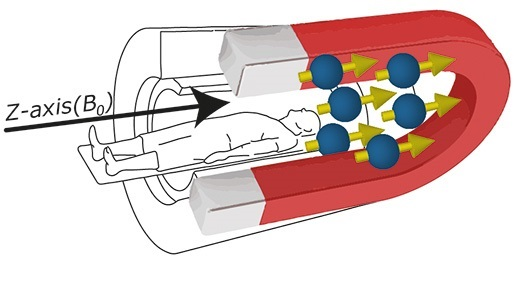
\includegraphics [width =13cm]{magnetic_field}
		\caption [Hydrogen atoms placed in the magnetic field]{Hydrogen atoms located in a human body placed in the strong magnetic field, $B_{0}$, generated by the MRI scanner, align to the direction of that field \cite{?}}
		\label{fig:magnetic_field}
	\end{figure}

In addition, atoms have an angular momentum making them precess about the magnetic field direction with a frequency $\omega_{0}$, called the \textit{Larmor frequency}, which is proportional to the field:   
\begin{equation}
\omega_{0} = \gamma{}B_{0}\:,
\label{eq:larmor}
\end{equation}
where $\gamma$ is the nuclei specific constant \textit{gyromagnetic ratio} (for hydrogen equal to 42.6\,MHz/T) and $B_{0}$ is the strength of the external magnetic field. This preccessional motion is is showed on Figure~\ref{fig:larmor}.

\begin{figure}
		\centering
		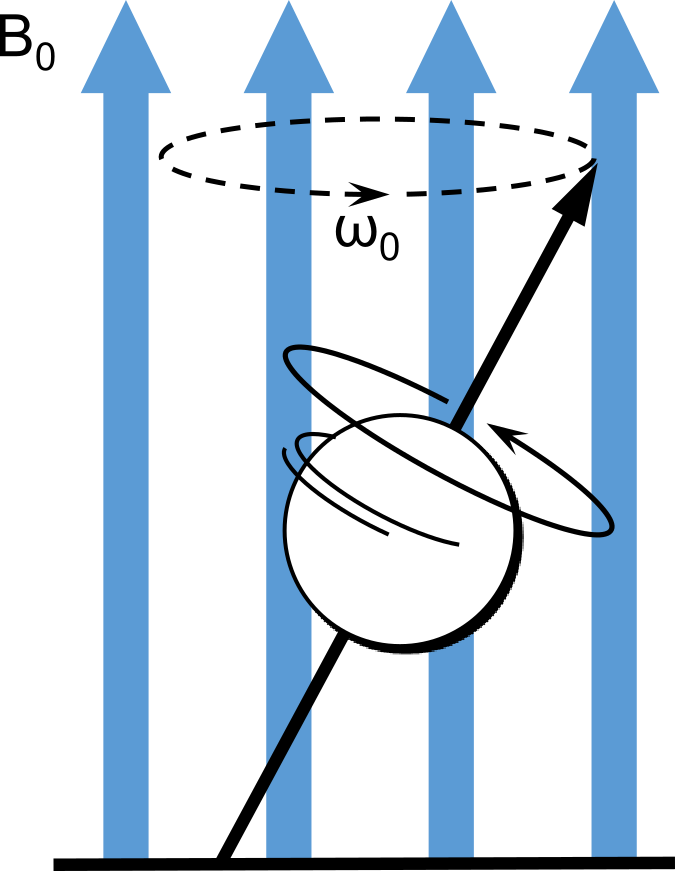
\includegraphics [width =6cm]{larmor}
		\caption [Precessional motion of the atom in the magnetic field]{Hydrogen atom placed in a strong magnetic field $B_0$ precesses about the direction of that field with the frequency $\omega_{0}$ \cite{?}}
		\label{fig:larmor}
	\end{figure}
Further, when the radio-frequency (RF) pulse equal to the Larmor frequency is applied perpendicularly to the magnetic field, the resonance occurs. The atoms absorb the energy, transits to the higher energy state and flip to the other position.
When the RF transmission is stopped, the atoms return to their equilibrium state (realign to the field $B_{0})$ releasing the energy as a radiation signal, referred to as \textit{free-induction decay} (FID) response signal, which is picked by MRI receiver. This return to equilibrium is called \textit{relaxation}. The relaxation time as well as the amount of the energy released strongly depends on the magnetic properties of the tissue, which means that every tissue generates different response signal. The MRI software analyses and processes obtained signal, which is a combination of numerous response signals from all excited atoms and generates the~image.       

During the MRI examination, the strength of the magnetic field produced by the scanner varies along the body, so that the Larmor frequency is different for different regions. By changing frequency of emitted RF, the appropriate part can be imagined. 

The typical MRI scanner consists of:
\begin{enumerate}
\item \textbf{The main field magnets}, which produces strong, uniform magnetic field polarizing the sample. Typical strength of the field of a clinical MRI scanner ranges between 0.2--3.0\, T, whereas research systems reaches values even up to 7.4\, T for Human and 21\, T for animal models.
\item \textbf{Shim coils.} In clinical practice, the main field magnets never produce perfectly uniform field so the shim coils adjusting its homogeneity have to be used.   
\item \textbf{Gradient coils} producing three secondary gradient magnetic fields in each of the x, y and z direction. In this way, the resonance frequency of protons varies as a function of position, which enables encoding the spatial position and imaging of thin anatomic slices \cite{hidalgo2010theory}.
\item \textbf{RF system}, task of which is to excite the hydrogen atoms and to receive their FID response signal
\item \textbf{The strong computer} controlling the system and processing the received combination of response signals.
\end{enumerate}

\subsection{\textit{T\textsubscript{1}} and \textit{T\textsubscript{2}} weighted images}

Although, there are few approaches of obtaining the contrast between different tissues in an image, utilizing different tissue properties, most widely used in clinical applications are these based on the relaxation of the magnetization. However, there are two kinds of relaxation, and thus two mechanisms of creating the MRI image can be listed.
\begin{description}
		\item [\textit{T\textsubscript{1}} weighted images] exploits spin–lattice relaxation, characterised by the time \textit{T\textsubscript{1}}, which describes the time required by excited atoms to return to the equilibrium state after it was altered by the RF pulse. This mechanism is shown in Figure \ref{fig:t1plot}. Sometimes the acquiring of T\textsubscript{1} weighted sequence is preceded by the injection of Gadolinium, paramagnetic contrast agent (CA), which  shortens time {T\textsubscript{1}} and appears very bright on the image. This property is especially useful while visualising vascular structures or brain tumours and abscesses blocking a blood supply.   
		
		\item [\textit{T\textsubscript{2}} weighted images] are based on spin-to-spin relaxation, described by the \textit{T\textsubscript{2}} indicating the time required by the nuclei response signal to decay after it has been created. \textit{T\textsubscript{2}} contrast is presented in Figure~\ref{fig:t2plot}. 
\end{description}
\begin{figure}[H]
\captionsetup[subfloat]{captionskip=0.5cm}
	\centering
	\subfloat[T1 plot]{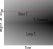
\includegraphics[height=6 cm]{t1plot}\label{fig:t1plot}}\hspace{1.5cm}
	\subfloat[T2 plot]{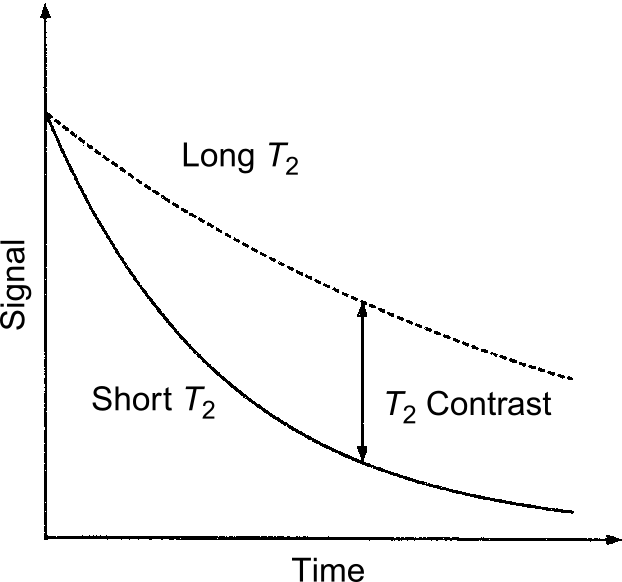
\includegraphics[height=6 cm]{t2plot}\label{fig:t2plot}}\\	
\vspace{0.5cm}
\caption{plots \cite{biomedical_hanbook_imaging}}
\label{fig:t1t2plot}
\end{figure}
Examples of the images acquired using described above two basic mechanisms are shown in Figure \ref{fig:t1t2}. 
The figure presents identical axial section of a healthy person's brain. In the \textit{T\textsubscript{1}} weighted  image on the left-hand side, one can notice bright ring of subcutaneous fat, which is due to its short spin–lattice relaxation time. Gray matter has longer \textit{T\textsubscript{1}} than white matter, so it appears darker. In the second picture, utilizing the \textit{T\textsubscript{2}} difference between tissues, cerebrospinal fluid in the ventricles appears very bright due to its long  \textit{T\textsubscript{2}}. \textit{T\textsubscript{2}} of the white matter is shorter that those of gray matter, which makes the latter one brighter. \textit{T\textsubscript{1}} and \textit{T\textsubscript{2}} weighted images are only two of the few contrast mechanisms used in  MRI and the choice of appropriate one strongly depends on the application and the region of interest under examination.

 
\begin{figure}
\captionsetup[subfloat]{captionskip=0.5cm}
	\centering
	\subfloat[T1 weighted image of a brain]{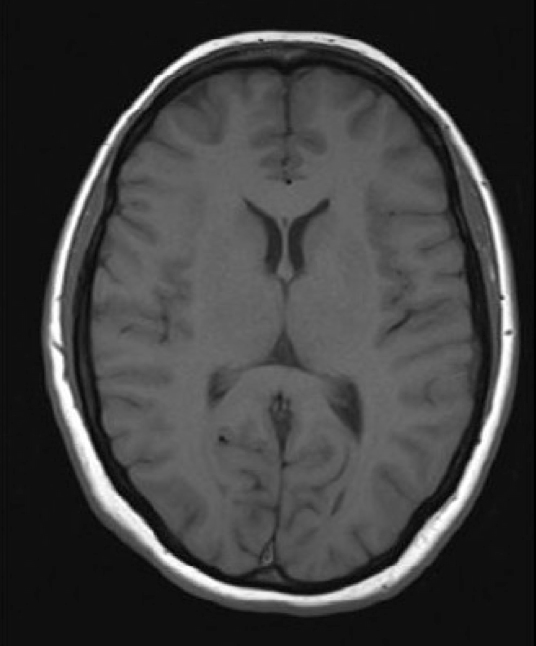
\includegraphics[height=7 cm]{t1}}\hspace{1.5cm}
	\subfloat[T2 weighted image of a brain]{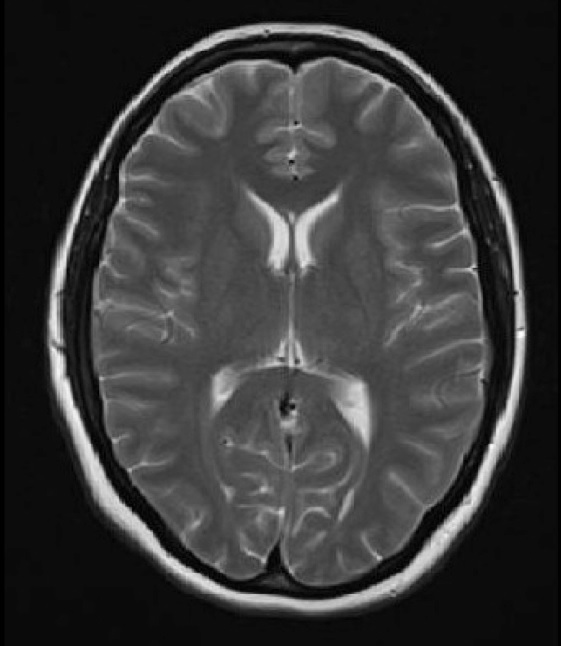
\includegraphics[height=7 cm]{t2}}\\	
\vspace{0.5cm}
\caption[Comparison of \textit{T\textsubscript{1}} and \textit{T\textsubscript{2}} weighted images]{Example MRI image of a brain of a healthy volunteer demonstrating T1 and T2 contrast}
\label{fig:t1t2}
\end{figure}

Currently MRI is one of the widest used medical imaging techniques applied in all parts of a body. It enables creating detailed anatomical images in axial, sagittal, coronal or even oblique plane. During MRI examination subsequent thin 2D \textit{slices} along chosen axis are produced, which makes it a tomographic imaging method. As a result, during imaging sequence, a large dataset is acquired, from which any anatomical section can be reconstructed or a 3D model of a region of interest can be assembled \cite {bushong2014magnetic}. Another advantage of MRI is not using any harmful ionizing radiation.
The clicical applications of MRI include diagnosis of blood vessel damages, multiple sclerosis, brain injuries, spinal cord injuries, brain strokes, blocked blood vessels, heart diseases, damages caused by a heart attack, bone infections, differnet kind of tumors and cancers and many more \cite{mriApplications}.

\section{DCE-MRI}
\textit{Dynamic Contrast Enhanced Magnetic Resonance Imaging} is basically the acquisition of multiple MRI scans, with addition of one extremely important component---the time domain \cite{jackson2005dynamic}. During the examination a Contrast Agent (CA) is injected in the peripheral vein into the bloodstream and the T1-weighted images are acquired with fast imaging technique. 
The passage of the tracer through the target tissue results in changes in signal intensities over the time.
The kinetics of the CA, so its is temporal and spatial distribution is strongly dependent on the physiological parameters such as tissue perfusion, volume of the extravascular and extracellular space and vessel permeability and thus the analysis of so obtained intensity changes as a~function of time, $S(t)$, provides important functional information \cite{bokacheva2008assessment, khalifa2014models}. 

\subsection{DCE-MRI analysis}
There are many methods of time-courses analysis obtained during DCE-MRI. In general, they can be divided into \begin{inparaenum}[(1\upshape)]\item qualitative \item semi-quantitative \item quantitative \end{inparaenum} ones \cite{barnes2012practical}.
All methods can be applied voxel-wise or to the whole Region of Interest~(ROI), where the average time-intensity curve is produced from the voxels values within the ROI \cite{khalifa2014models}. 

\subsubsection{Qualitative analysis}
In traditional approach, the evaluation of the time-intensity curves is performed by experienced observer via subjective visual inspection, who's task is to classify the curve to one of the three predefined enhancement patterns. This three \textit{templates} are shown on Figure~\ref{fig:patterns}.  
Type~I, defines a shape characterized by the gradual increase of the signal intensity during the whole acquisition time. In type~II, after the initial peak, the plateau occurs---the curve remains relatively constant. Type~III is associated with the decrease in signal intensity after the peak signal intensity \cite{barnes2012practical}.
In this way, i.e the tumour can be distinguished from the healthy tissue.

Although the qualitative analysis is a very convenient one as it does not require any additional data and calculation, its  major disadvantage is not delivering any quantitative parameters and being fully dependent on the observer's experience. \vspace{10pt}
 
\begin{figure}[b!]
		\centering
		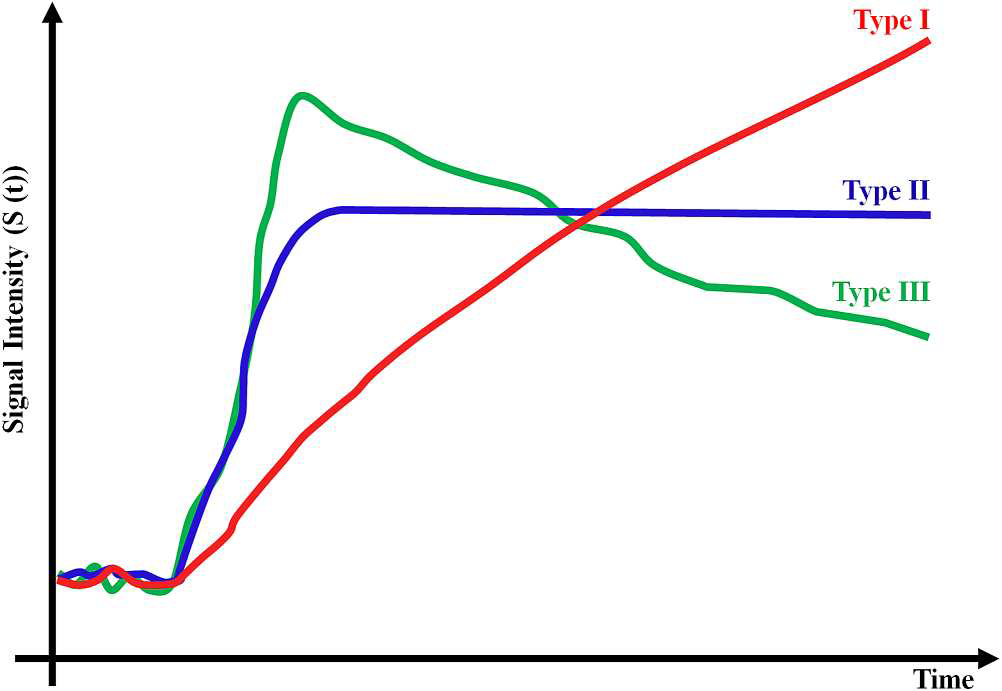
\includegraphics [width =9cm]{dcemri_patterns}
		\caption [DCE-MRI enhacement patterns]{Different DCE-MRI enhacement patterns \cite{khalifa2014models}}
		\label{fig:patterns}
	\end{figure}

\subsubsection{Semi-quantitative analysis}
The semi-quantitative analysis incorporates calculation of parameters directly from the time-intensity curve characterizing its shape \cite{khalifa2014models, barnes2012practical}. Several examples of the parameters include \textit{onset time} ($T_o$), \textit{maximum signal intensity} ($S_m$), \textit{peak enhancement} ($\Delta S$), \textit{time to peak} ($T_p$), \textit{wash-in slope}, \textit{wash out slope}, \textit{average plateau},  \textit{Area Under the Curve} (AUC) or \textit{Initial Uptake Area Under the Curve} (IAUC) \cite{khalifa2014models}. Listed parameters are depicted in Figure~\ref{fig:parameters}. 

As in the case of previous method, the ease of the calculations performed directly from the curve is its biggest advantage.  However obtained empirical parameters in some way correlate with tissue physiology, i.e. increased vascular density
or permeability usually increases the wash-in slope, AUC, and peak enhancement,
in the same time decreasing the time to peak, it is difficult to relate them directly to some particular physiological quantities \cite{barnes2012practical}.
\begin{figure}[h!]
		\centering
		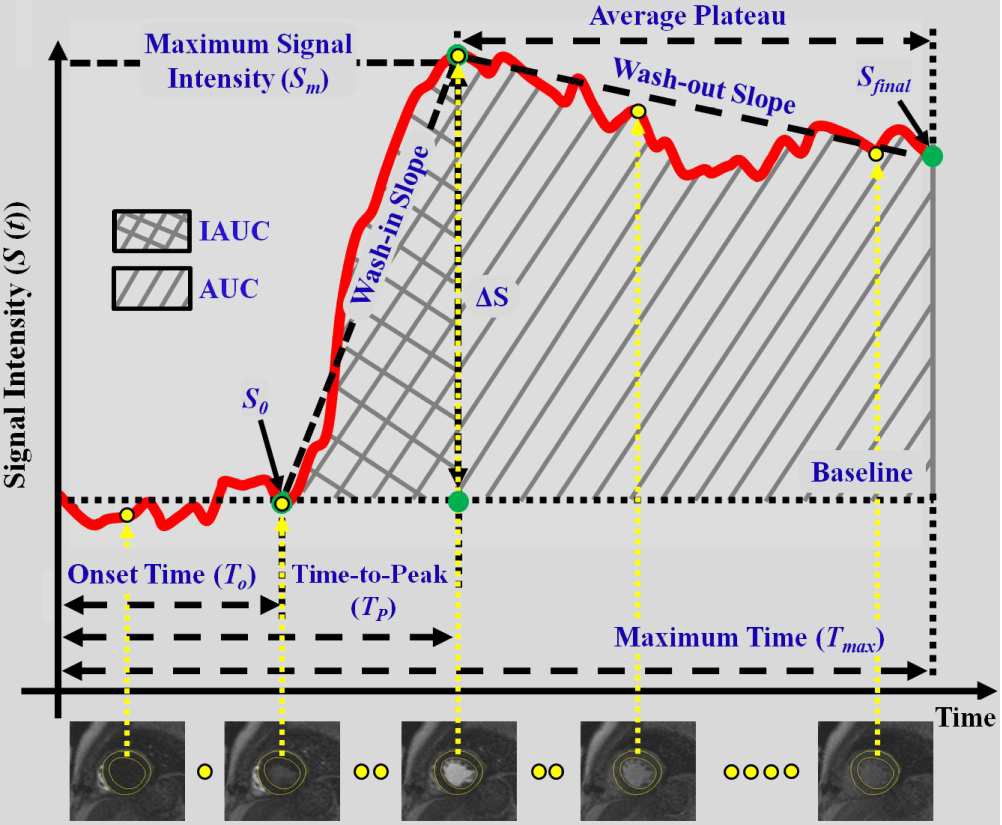
\includegraphics [height=7.5cm, width =10cm]{semi}
		\caption [Sample paramterers used in semi-quantitative DCE-MRI analysis]{An example of the time-intensity curve, $S(t)$, with depicted metrics explored  in semi-quantitative DCE-MRI analysis. Note that $S_0$ is the signal intensity before CA arrival whereas $S_{final}$ is the intensity registered in the last temporal point at the end of the experiment $T_{max}$ \cite{khalifa2014models}}
		\label{fig:parameters}
	\end{figure}



\subsubsection{Quantitative analysis}
Quantitative assessment of the $S(t)$ curve is surely the most sophisticated one. Not only one has to convert the signal-intensity curve into  
The issue of the pharmacokinetic modelling in details is described in Chapter~{\ref{chapter:pk}.
\subsection{DCE-MRI applications}
There is no doubts that obtaining important both structural and functional information in a single imaging session is one of the biggest advantage of Dynamic Contrast Enhanced MRI.

% Chapter - Principles of pharmacokinetic modelling
\chapter{Pharmacokinetic modelling}
\label{chapter:pk}

The ideal output obtained from DCE-MRI analysis would be some reliable quantitative physiological parameters of the tissue under examination. 

PK models have very wide clinical application: from estimating the optimal drug dose to determining safe working environment while working with toxins  \cite{gerlowski1983physiologically}.
Given the fact that the contrast agent used in DCE-MRI examination can be considered as a substance flowing through the organism, pharmacokintetic modelling can also be used in analysis of so obtained data.   
This approach, called the parametric one, is based on fitting mathematical model to acquired tissue concentration time courses. In this way, the quantitative parameters can be assessed, which cannot be overestimated while evaluating the tissue function. 


\section{Arterial Input Function}
All PK models require the qquistition Arterial Input Function


\begin{comment}
The time-dependent distribution and disposition of a substance in a living system can be described by phamacokinetic (PK) models~\cite{gerlowski1983physiologically}. They aim to characterise a physiologic system by decomposing them into interacting compartments. Every of them is a homogenous, well-mixed space with the uniform tracer distribution \cite{PMID:20540902}.









The compartment PK models decribe complex
blood-tissue exchanges and their theory
is based on the differential mass balance equations
[29]. An example of the system decribed
by two compartments is presented on Figure 5.
	


\end{comment}

\begin{figure}
		\centering
		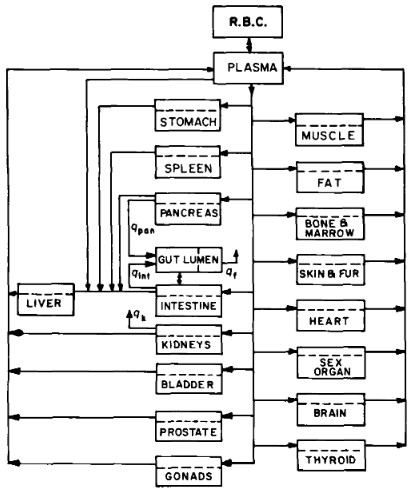
\includegraphics[height = 10cm]{scheme}
		\caption [DCE-MRI enhacement patterns]{Different DCE-MRI enhacement patterns \cite{khalifa2014models}}
		\label{fig:pk_draft}
	\end{figure}

% Chapter - Implementation of the method
\chapter{Implementation}

\section{Materials and methods}
\subsection{DCE-MRI aquisition}
The dataset used in this project consists of forty DCE-MRI sequences. Each of the 20 healthy, non-smoking participants underwent two MRI examination at a~time interval of 7 days.
A gadolinium-based CA GdDOTA (Gadoteric Acid) at a dose of 0.025\,mmol/kg was administrated as a bolus injection at 3\,ml/s.
The data were acquired on 32 channel 1.5 T whole-body scanner (Siemens Magnetom Avanto \cite{simens}).
The  images covering kidneys and aorta were continuously acquired every 2.3 s for approximately 6 min in coronal-oblique plane.
Each of 74 time volumes consisted of 30 slices.
The aquisition matrix was 192\,x\,192 whereas the voxel size was equal to 2.2\,x\,2.2\,x\,3\,mm$^3$
More information about aquisition of DCE-MRI data used in this project can be found in \cite{eikefjord2017dynamic}.
The few frames of the sample raw DCE-MRI sequence is shown in Figure~\ref{fig:set}.



\begin{figure}

\captionsetup[subfigure]{labelformat=empty,textformat=simple}
	\centering
	\subfloat[\textit{T} = T0]{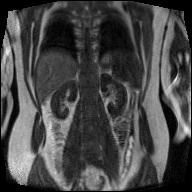
\includegraphics[height=0.24\linewidth]{img/preview/00}}\hspace{0.005\linewidth}
		\subfloat[\textit{T} = T9]{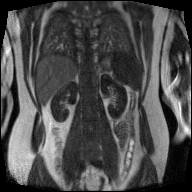
\includegraphics[height=0.24\linewidth]{img/preview/09}}\hspace{0.005\linewidth}
			\subfloat[\textit{T} = T12]{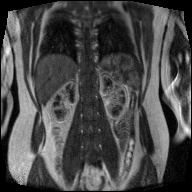
\includegraphics[height=0.24\linewidth]{img/preview/12}}\hspace{0.005\linewidth}
			\subfloat[\textit{T} = T16]{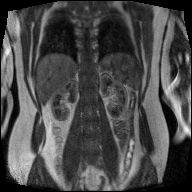
\includegraphics[height=0.24\linewidth]{img/preview/16}}\vspace{-4pt}
			
			\subfloat[\textit{T} = T18]{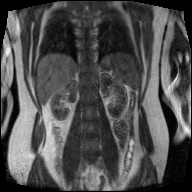
\includegraphics[height=0.24\linewidth]{img/preview/18}}\hspace{0.005\linewidth}
		\subfloat[\textit{T} = T22]	{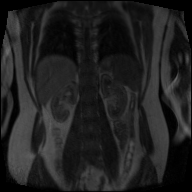
\includegraphics[height=0.24\linewidth]{img/preview/22}}\hspace{0.005\linewidth}
		\subfloat[\textit{T} = T26]{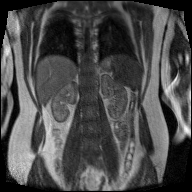
\includegraphics[height=0.24\linewidth]{img/preview/26}}\hspace{0.005\linewidth}
			\subfloat[\textit{T} = T30]{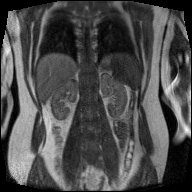
\includegraphics[height=0.24\linewidth]{img/preview/30}}\vspace{-4pt}

			\subfloat[\textit{T} = T34]{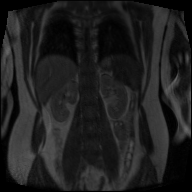
\includegraphics[height=0.24\linewidth]{img/preview/34}}\hspace{0.005\linewidth}
		\subfloat[\textit{T} = T39]	{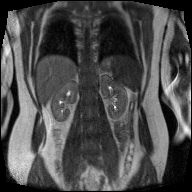
\includegraphics[height=0.24\linewidth]{img/preview/39}}\hspace{0.005\linewidth}
	\subfloat[\textit{T} = T55]{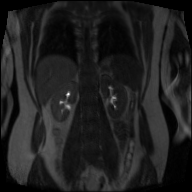
\includegraphics[height=0.24\linewidth]{img/preview/55}}\hspace{0.005\linewidth}
	\subfloat[\textit{T} = T73]{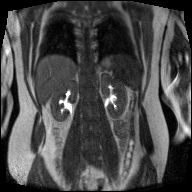
\includegraphics[height=0.24\linewidth]{img/preview/73}}
\vspace{0.5cm}
\caption[Sample DCE-MRI sequence.]{Sample DCE-MRI sequence}
\label{fig:set}
\end{figure}


\subsection{GFR reference values}
Next to the DCE-MRI examinations, the participant had their GFR assessed by two commonly used in clinical practice chemical methods: the Serum-creatinine (SCr) and iohexol GFR tests.  

The clinical characteristic of the participants is included in Table~\ref{tab:participants}



\begin{table}[h!]
\centering
\caption[Clinical characteristic of the participants]{Clinical characteristic of the participants. Taken from \cite{eikefjord2017dynamic}}
\label{tab:participants}
\begin{threeparttable}
\rowcolors{2}{}{beaublue!50}
\renewcommand{\arraystretch}{1.25}
\begin{tabular}{m{8cm} m{2.25cm}}
	\hline

 	Participants & 20\\
  	Gender (female/male) &16/4\\
  	Age (years) & 25 (20---38)\\
  	Height [m] & 1.71 $\pm$ 00.7\\
  	Weight [kg] & 66.2 $\pm$ 8.7\\
  	Body mass index (BMI) [kg/m\textsuperscript{2}] & 22.6 $\pm$ 2.1\\
  	Body surface area (BSA) [m\textsuperscript{2}]& \\
  	Iohexol GFR [ml/min/m\textsuperscript{2}] &103 $\pm$ 10\\
  \hline

\end{tabular}
\begin{tablenotes}%
\footnotesize{}%
\item Values in parentheses are ranges.
\item Plus minus values are means $\pm$ Standard Deviations (SD).
    \end{tablenotes}
	\end{threeparttable}
\end{table}



\subsection{Image processing and analysis}
\subsubsection{Motion correction}
One of the first fundamental problem encountered during DCE-MRI analysis is misalignment of 3D volumes across time slices. This misalignment of organs is a result of the patiens's respiratory motion as well as the heartbeat and bowel peristalsis and is unavoidable during examination. Studies have shown that even slight misalignment can lead to significant differences in intensity time-courses \cite{KidneySubsegmentation} and thus, motion correction of time series is essential for further analysis.

In order to remove motion artifact, all files were motion-corrected across time points. For this purpose R programming language for statistical computing and graphics was used \cite{R} together with the package ANTsR \cite{ANTsR}, which provides quantification tools for biomedical images. As an initial step, for every time series, the algorithm extracted 3D volumes. Each extracted volume corresponded to data obtained in one time point. Next, the average image of the temporal volumes was calculated, which was treated as a mask for image registration. Every temporal volume was then aligned to the mask and at the end they were combined back together into 4D time series.

\subsubsection{Pelvis removal}
Due to the fact that glomelular filtration takes place in renal renal parenchyma, pelvis had to be removed from further analysis. 

Resulting from the physiology of the process, the three renal compartments (cortex, medulla, pelvis) can be distinguished from each other on the basis of their time courses, as shown on Figure~\ref{fig:timecourses}. Depending on the compartment, the rapid enhancement of the signal occurs in different period, which makes the shapes of the time intensity curves very unique.
From the \ref{fig:timecourses} it can be seen that the biggest variation is observed between pelvis and two other renal compartments.    Consequently, it can be separated by unsupervised clustering. 

\begin{figure}[H]
	\centering
	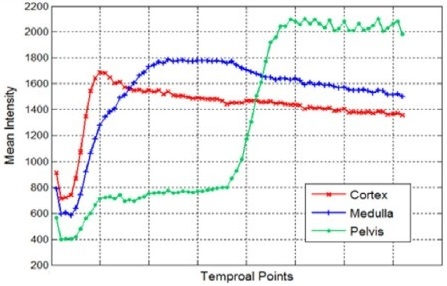
\includegraphics{img/timecourses}
	\caption{Kidney compartments timecourses  \cite{KidneySubsegmentation}}
	\label{fig:timecourses}
\end{figure}

First of all, every of the the voxel belonging to the label of the kidney was described by the vector of seventy-four features as follows:
\begin{equation}
\label{eq:voxel}
\mathbf{v_{ijk}} = [S_{T0},\; S_{T1},\;...\;,\; S_{T72},\; S_{T73}],
\end{equation}
where $S_{Tn}$ is the value of signal intensity in the time point $n$.

However, feature space of seventy-four dimensions is way too much for further analysis. High dimensionality of raw DCE-MRI data results in computational complexity, and thus memory and time consumption as well as numerical problems. What is more it contains a lot of noises \cite{KidneySubsegmentation}. To overcome this problems, the \textit{Principal Component Analysis} (PCA) \cite{wold1987principal} was applied.

PCA is a statistical procedure, which transforms the number of related features into smaller set of uncorrelated variables  \cite{pca}. These so called \textit{Principal Components} (PCs) are a linear combination of the original variables \cite{dunteman1989principal}. As a result, after rotating the feature space, the first PC contains most variance, the last one the least and so on. In this way the dominant patterns are extracted while the noises are reduced~\cite{wold1987principal}. Further, every of the PC is characterised by a ratio of \textit{explained variance}, which indicates the portion of the dataset’s variance lying along the axis of each PC~\cite{handson}.

Applying the theory to practice, each voxel belonging to the kidney, initially described by forty-four features was described by a number of PCs:
\begin{equation}
\label{eq:voxelpca}
\mathbf{v_{ijk}} = [PC1,\; PC2,\;...\;,\; PCn]  
\end{equation}
The amount of PCs, $n$, was chosen as a minimum number of dimensions required to preserve 95\% of the data's total variance so that that the sum of the explained variances of  $n$ PCs was equal to at least 0.95 (usually between 4---6 PCs). The visual representation of the feature space with first three dimensions (PCs) for sample kidney is shown in Figure~\ref{fig:pca_plot}. Note that for better understanding, the clusters were already marked with different colors. 

\begin{figure}[H]
		\centering
		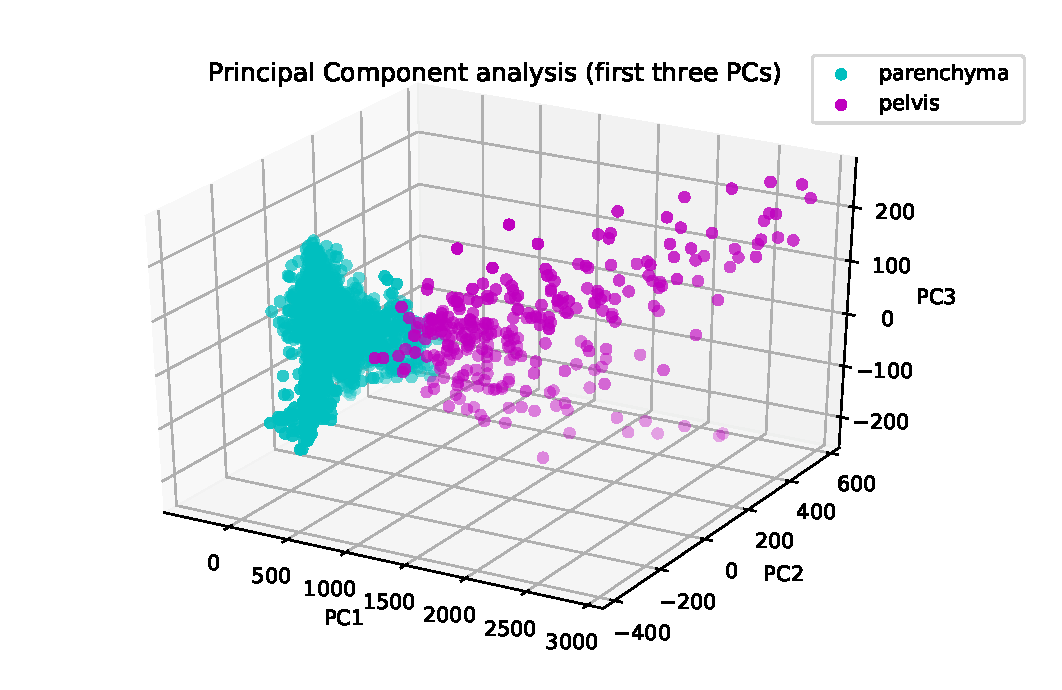
\includegraphics [height = 10cm]{pca}
		\caption [Principal Component Analysis for sample kidney]{Principal Component Analysis for sample kidney. The values in brackets are the ratios of explained variance for the given PCs. Note that the number of PCs was reduced to three for visualisation purpose}
		\label{fig:pca_plot}
	\end{figure}

To the dimensionally reduced data, the \textit{k-means clustering} \cite{kmeans} was applied in order to separate voxels into two groups: pelvis and renal parenchyma. 
The k-means is an unsupervised clustering algorithm aiming to divide the data into groups so that the diversity between the groups is maximised whereas the similarity within the single group is maximised. 

Given a data set $X=\{ \vec{x_1}...\vec{x_n}$\} in $m$-dimensional space (what actually corresponds to the $m$ features of a sample) the algoritm's objective is to minimize the square error function given by:

\begin{equation}
	\label{eq:kmeans}
	J = \sum_{j=1}^{k}\sum_{i=1}^{n}(||x_i-c_j||)^2,
\end{equation}
where $||x_i-c_j||$ is  the Euclidean distance between a data point $x_i$ and the cluster centre $c_j$ of $k$ predefined clusters. It is achieved by the steps summarised in Algorithm~\ref{alg:kmeans}.

\vspace{16pt}
\begin{algorithm}[H]
\footnotesize
    \SetKwInOut{Input}{Input}
    \SetKwInOut{Output}{Output}
    \SetKwFunction{RandomlyChooseCentroids}{RandomlyChooseCentroids}
    \SetKwFunction{CalculateMeanOfPointsInCluster}{CalculateMeanOfPointsInCluster}
    \SetKwData{Centroids}{$(\vec{c_1}...\vec{c_k})$}
    \SetKwFunction{argminDistance}{argminDistance}
    
	\Input{number of clusters $k$,\\ set of points in $m$-dimensional space: $X=\{ \vec{x_1}...\vec{x_n}$\}}
	
    \Output{set of cluster labels of $X$: $L = \{l(\vec{x_i})\;i \in\{1...n\}\}$ ,\\ coordinates of cluster centroids: \Centroids}
    
    \BlankLine
    \BlankLine
    
    
	\DontPrintSemicolon
	\Centroids $\leftarrow$ \RandomlyChooseCentroids{$k$, $X$} \Centroids$\in X$\;
    
	\Repeat{none of \Centroids changes}{
\tcc {assign each data point to the closest centroid on the basis of Euclidean distance}
$l(\vec{x_i})\leftarrow$\argminDistance($\vec{x_i}$, $\vec{c_j}$) $j \in\{1...k\}$ \\
\Centroids$\leftarrow$  \CalculateMeanOfPointsInCluster{}  \tcc*{recalculate centroids} 
}
	\Return{$L$ , \Centroids} \tcc*{points divided into clusters} 
    
    
    \SetAlgoCaptionSeparator{.}
    \caption{K-means clustering}
    \label{alg:kmeans}
\end{algorithm}

\vspace{16pt}
To segment the kidney, the k-means algorithm was initiated with two clusters, $k$~=~2 and performed for points (kidney voxels) in ten-dimensional space (10 PCs).

Furter, for each of the identified clusters, the average time point, $T_{max}$ in which signal intensity reaches its maximum was calculated. 
Following the assumption that $T_{max\_pelvis}>T_{max\_parenchyma}$, the cluster with greater $T_{max}$ was marked as the pelvis and removed from the \textit{Region of Interest} (ROI).
The average time-intensity curves for two detected clusters in k-means clustering algorithm for sample kidney are presented in Figure~\ref{fig:clusters}. On can easily note the wash in phase in pelvis takes place much later than in renal parenchyma. The results of the segmentation in turn are shown in Figure \ref{fig:segmentation}.  


\begin{figure}[H]
%\captionsetup[subfloat]{captionskip=0.5cm}
	\centering
	{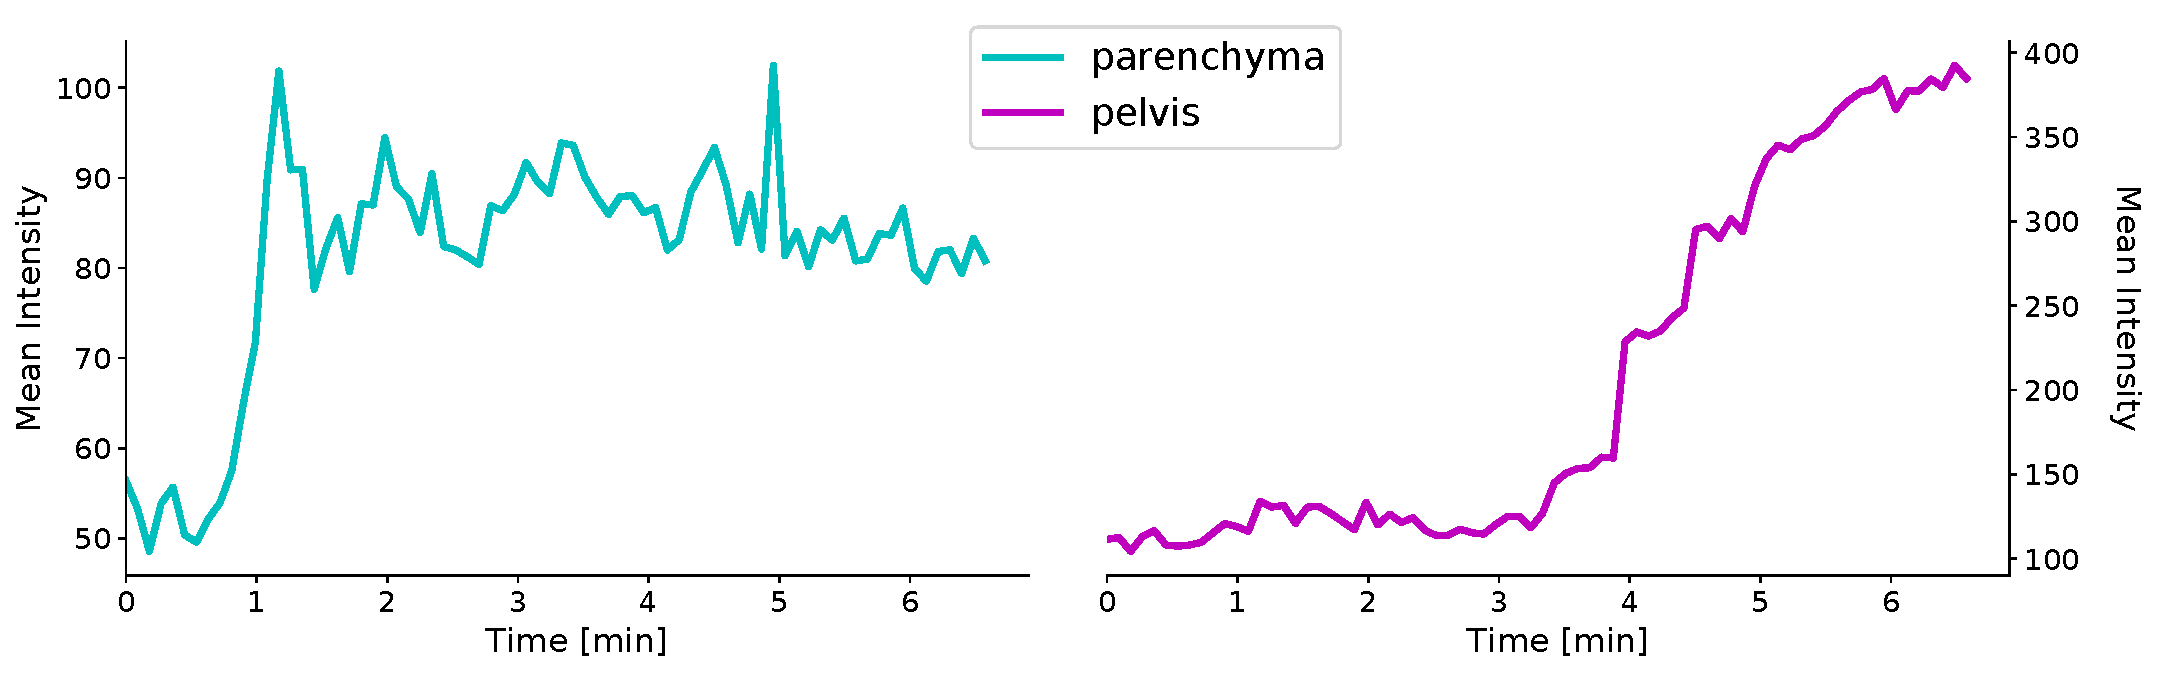
\includegraphics[width = \textwidth]{clusters}\label{fig:tcluster1}}
	
\caption[Average time courses for two clusters detected in k-means algorithm]{Average time courses for two clusters detected in k-means algorithm performed for sample kidney}
\label{fig:clusters}
\end{figure}

\begin{figure}[H]
\captionsetup[subfloat]{captionskip=0.5cm}
	\centering
	\subfloat[\textit{T1}-weighted image of a brain]{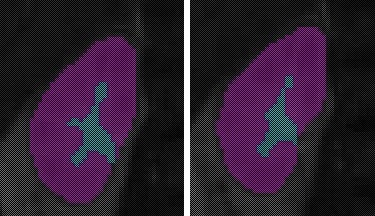
\includegraphics[width=0.48\textwidth ]{kidney_pelvis}}\hspace{0.02\textwidth}
	\subfloat[\textit{T2}-weighted image of a brain]{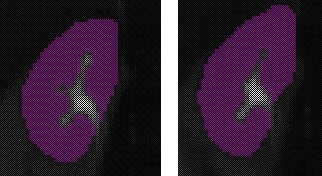
\includegraphics[width=0.48\textwidth]{no_pelvis}}\\	
\vspace{0.5cm}
\caption[Comparison of \textit{T\textsubscript{1}}- and \textit{T\textsubscript{2}}-weighted images]{Note that the images were normalised within extracted slices for better visualisation}
\label{fig:segmentation}
\end{figure}



\subsubsection{Concentration-time curves}
For each of the kidney, as well as for the aorta, the mean intensities in each time point were calculated. 

Assuming the linear relation between tracer concentration and signal intensity $S(t)$ \cite{lim2013prediction}, the tracer concentration can be expressed as:


\begin{equation}
	\label{eq:conversion}
	C(t) = S(t)-S(0),
\end{equation}
  
where $S(0)$ is the baseline signal. In order to determine S(0), the time point before rapid signal drop had to be found  as marked on Figure \ref{fig:point}.
%%% Experimenting with two methods, not decided yet %%%%

\textbf{First method:} To do so, for the time course under analysis, the time point in which the derivative of the function reaches the maximal value was selected. 

 

\subsubsection{Pharmacokinetic modelling}



\section{Results}








\begin{comment}

%\begin{equation}
%	\label{eq:extended_toft}
%	\nonumber C_{t}(t) = v_pC_p(t)+ K_{trans}\int_{0}^{t}C_p(t')e^{-(K_{trans}/v_e)(t-t')}dt', 
%\end{equation}
%where:\\
%$v_e$ - fractional volume of the extravascular extracellular space\\
%$v_p$ - fractional plasma volume\\
%$K_{trans}$ - transfer constant\\
%$C_{t}$ - Tissue concentration\\
%C_{p}$ - Concentration in aorta (AIF)


 
\subsection{Manual labelling of kidneys and aorta} 
\label{subsec:labelling}
In the next step, labels of both left and right kidney were created. For this purpose, 3D volumes were extracted for every time frame and the image with maximal signal enhancement was chosen (usually between 12--17 time slice). On this image, left and right kidney were manually delineated in coronal plane using ITK-Snap software \cite{itk-snap}. Additionally, few voxels of aorta (15--20) were labelled. So obtained labels were then propagated across the time points. All further analysis was implemented in Python programming language v. 3.6 \cite{python}.  
 


\newpage
\subsection{Pharmacokinetic modelling}
The time-dependent distribution and disposition of a substance in a living system can be described by phamacokinetic (PK) models~\cite{gerlowski1983physiologically}. They aim to characterise a physiologic system by decomposing them into interacting compartments. Every of them is a homogenous, well-mixed space with the uniform tracer distribution \cite{PMID:20540902}.




PK models have very wide clinical application: from estimating the optimal drug dose to determining safe working environment while working with toxins  \cite{gerlowski1983physiologically}.
Given the fact that the contrast agent used in DCE-MRI examination can be considered as a substance flowing through the organism, pharmacokintetic modelling can also be used in analysis of so obtained data.   
This approach, called the parametric one, is based on fitting mathematical model to acquired tissue concentration time courses. In this way, the quantitative parameters can be assessed, which cannot be overestimated while evaluating the renal function. 
 

\begin{figure*}[t]
	\centering
	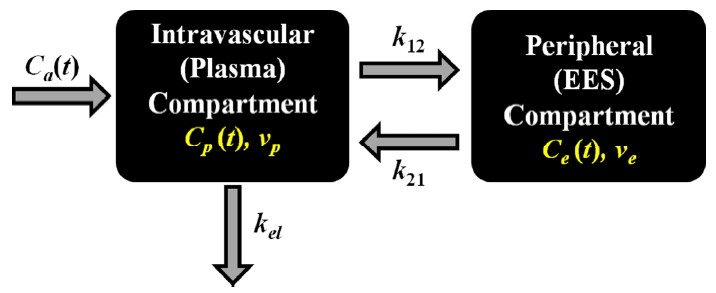
\includegraphics[width = 11cm]{img/diagram2}
	\caption{An example two compartment model \cite{khalifa2014models}.}
	\label{fig:diagram2}
\end{figure*}

The compartment PK models decribe complex blood-tissue exchanges and their theory is based on the differential mass balance equations \cite{sourbron2011tracer}. 
An example of the system decribed by two compartments is presented on Figure \ref{fig:diagram2}.


\subsubsection{Concentration time courses}
  

All PK models used during DCE-MRI analysis require determining both the tissue, $C_t(t)$, and blood plasma, $C_p(t)$, concentration as a~function of time. In our case, the $C_t(t)$ is the mean concentration in renal parenchyma, whereas the
$C_p(t)$, or so called arterial input function (AIF), is a concentration in a blood vessel feeding the kidney (aorta) \cite{khalifa2014models}.  



\begin{figure*}
	\centering
	\subfloat[Kidney time course]{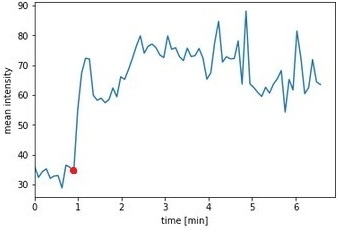
\includegraphics[width=6 cm]{img/timecourse_kidney}}\quad
	\subfloat[Aorta time course]{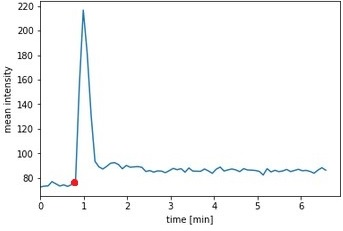
\includegraphics[width=6 cm]{img/timecourse_aorta}}\\		
\caption{Sample average time-courses for renal parenchyma (a) and aorta (b). The last point of baseline is marked with red dot.}
\label{fig:point}
\end{figure*}

Obtained time-concentration curves were then fitted to the described in the next sections PK models.



\subsubsection{Toft's model}
The two compartment Toft's model \cite{tofts1991measurement} assuemes the diffusion of the tracer from the blood plasma at rate specified by the transfer constant $K_{trans}$ $(min^{-1})$ and returns at the rate $k_{ep} = K_{trans}/v_e$ $(min^{-1})$. In this model the assumption $C_t(t) = v_eC_e(t)$ is made, which means that plasma contribution is neglected. The blood plasma concentration $C_p$ is specified by AIF. According to the Toft's model the CA concentraion is specified by the formula:
 
\begin{equation}
	\label{eq:toft}
	C_{t}(t) = K_{trans}\int_{0}^{t}C_p(t')e^{-(K_{trans}/v_e)(t-t')}dt'  
\end{equation}

\subsubsection{Extended Toft's model}
While the Toft's model neglects intravascular contribution assuming weak vascularization of the tissue, the Extended Toft's model \ref{tofts1997modeling} does take it into account. The tissue concentration is described by the formula:
\begin{align}
	\label{eq:extended_toft}
	\nonumber C_{t}(t) &= v_pC_p(t)+\\ 
	&+ K_{trans}\int_{0}^{t}C_p(t')e^{-(K_{trans}/v_e)(t-t')}dt', 
\end{align}
where $v_p$ is the fractional plasma volume. 

In Toft's and extended Toft's models the free parameters $K_{trans}$, $v_e$ and $v_p$ are estimated by fitting the model to obtained in DCE-MRI examinations time concentration curves.  

\subsubsection{Patlak plot}
Another proposed approach is the graphical one called Patlak plot \cite{patlak1983graphical}. Patlak plot neglects $k_{ep}$ due to the low permeability and short examination time. As a result tissue concentration is expressed as:

\begin{equation}
	\label{eq:patlak}
	C_{t}(t) =v_pC_p(t) + K_{trans}\int_{0}^{t}C_p(t')dt'  
\end{equation}
The above equation is the linearised as:
\begin{equation}
	\label{eq:patlak_lin}
	Y = K_{trans}X +v_p,  
\end{equation}
where $Y=C_t(t)/C_p(t)$ and $X=\int_{0}^{t}C_p(t')dt'/C_p(t)$. The free parameters $K_{trans}$ an $v_p$ can be then estimating by constructing a linear plot and calculating its slope and intercept respectively.

\subsubsection{GFR estimation}
Having calculated the $K_{trans}$ parameter the glomelural filtration rate can be computed according to the formula:
\begin{equation}
	\label{eq:gfr}
	GFR = K_{trans}V_{parenchyma}(1-H_{ct}) 
\end{equation}

\begin{figure*}
	\centering
	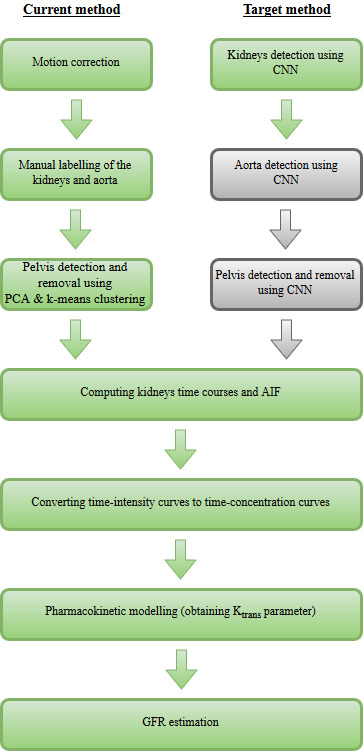
\includegraphics[height = 18cm]{img/methods}
	\caption{}
	\label{fig:methods}
\end{figure*}

\end{comment}


% Chapter - Summary
\chapter{Summary}

%\addcontentsline{toc}{chapter}{Summary}

The main purposes of this thesis were, firstly, to design a library in Python programming language for pharmacokinetic modelling from DCE-MRI images, which is to be incorporated into the fast method of GFR estimation, and secondly, to compare the performance of the few PK models for application of assessing renal function and to examine whether any of them can be considered accurate and precise enough to be used in the target method.

As a first step, the DCE-MRI sequences were registered in a time domain and both kidneys as well as aorta were manually labelled. Next, the renal pelvis was removed from the kidneys' labels on the basis of voxels' intensity time courses. For this purpose the PCA together with k-means clustering was applied. Subsequently, the average time-intensity curves were obtained for both kidneys and aorta. The signal intensity was converted into concentration by finding the temporal point, at which positive $S'(t)$ reaches the maximum value. So obtained concentration time courses were then fitted to four pharmacokinetic models: Tofts Kermode, Extended Tofts Kermode, Rutland Patlak and two-compartment exchange models. Finally, on the basis of the obtained parameters the SKGFR as well as total GFR were calculated and compared with two chemical methods. 
  
The developed algorithm was tested on the DCE-MRI sequences of ten different participants. Dice similarity coefficient of the pelvis segmentation was equal to DSC~=~0.86\,$\pm$\,0.06. For each of the sequence the pelvis was removed correctly without the need of manual correction. Regarding the performance of different PK models, the obtained results show that 2CXM is the most accurate and precise one and gives results comparable with those of the SCr blood test, which is a commonly used clinical method. What is more, the obtained $P30 = 100\%$ for this model proves that its estimation is sufficient to be used in clinical use.   

All in all, the thesis was a success. An important contribution is creating the module in Python, which will be used in further research on fast method of GFR estimation.  
On the basis of the drawn conclusions of practical tests the 2CXM model can be applied as a final step of the target method.

The source code is available at \underline{\url{https://github.com/KasiaSprawka}}.


% Bibliography
\newpage
\phantomsection \label{sec:References}
\addcontentsline{toc}{chapter}{References}
\begin{spacing}{1.2}
\bibliographystyle{ieeetr}
\bibliography{./tex/references}
\end{spacing}

%List of Figures
\newpage
\phantomsection \label{sec:ListOfFigures}
	\addcontentsline{toc}{chapter}{List of Figures}
	\begin{spacing}{1.0}
		\listoffigures
	\end{spacing}
	
%List of Tables
\newpage
\phantomsection \label{sec:ListOfTables}
	\addcontentsline{toc}{chapter}{List of Tables}
	\begin{spacing}{1.0}
		\listoftables
	\end{spacing}




%----------------------------------------------------------------------------------------
%	Section: Methods
%----------------------------------------------------------------------------------------
\newpage
%\section{Methods}
%\label{sec:Methods}
%\chapter{Materials and methods}
\section{DCE-MRI renography}
When the contrast agent is injected into the bloodstream, is starts its journey via the organism. It travels  through the abdominal aorta, which branches  into the left and right renal arteries supplying the kidneys with the blood.  

First, the CA reaches the renal cortex, where a portion of it is filtered by the glomerulus from the blood to the Bowman's capsule in the process of glomerular filtration. Next, it is passed by the renal tubule to the renal medulla to finally be collected by the collecting system.   
Chemicals such as gadolinium-based markers used in DCE-MRI that are freely filtered but neither reabsorbed nor secreted by the kidneys can be used for estimating the glomerular filtration rate in quantitative DCE-MRI analysis.
\begin{comment}
This chapter describes in details the implemented method of the quantitative analysis of the kidney's function. Firstly, the subsequent steps of image processing and analysis are presented and the, the performance of the chosen PK models is compared. The aim is to chose the model, which would be the best for GFR estimation and to draw a conclusion whether it can be considered a robust and reliable method for future applications. 
\end{comment}

This part of the thesis describes in details the implemented method of the quantitative analysis of the kidney's function from DCE-MRI. The chapter leads the reader through the subsequent steps of image processing and analysis to finally compare the performance of the chosen PK models. The aim is to choose the model, which allows for obtaining the best results for GFR estimation on the given data and to draw a conclusion if it can be considered a robust, reliable method for the future applications. 

\section{DCE-MRI acquisition}
The dataset used in this project consists of forty DCE-MRI sequences. Each of the twenty healthy, non-smoking participants underwent two MRI examinations at a~time interval of 7 days.
Gd-DOTA (\textit{gadoteric acid}), which is a gadolinium-based CA,  at a dose of 0.025\,mmol/kg was administrated as a bolus injection at 3\,mL/s in an antecubital vein followed by a 20\,mL saline flush.
The examinations were performed on the 32 channel 1.5\,T whole-body scanner (Siemens Magnetom Avanto \cite{simens}) with a gradient strength\,=\,45\,mT/m and slew rate\,=\,200\,mT/m/ms using a~standard six-channel body matrix coil and table-mounted six-channel spine matrix coil for signal reception.
The 74 volumes, each consisting of 30 slices, covering the kidneys and the aorta were continuously acquired every 2.3\,s for approximately 6\,min in coronal-oblique plane.
The acquisition matrix was 192\,$\times$\,192 whereas the voxel size was equal to 2.2\,$\times$\,2.2\,$\times$\,3\,mm$^3$.
The parameters of the used spoiled gradient recalled 3D FLASH pulse-sequence were: echo time, $TE=0.8$\,ms, repetition time, $TR=2.36$\,ms, flip angle, $\alpha= 20^{\circ}$.

More information about the acquisition of DCE-MRI data used in this project can be found in \cite{eikefjord2017dynamic}.
A few frames of the sample raw DCE-MRI sequence are shown in Figure~\ref{fig:set}.
\newpage

\begin{figure}[H]
%\vspace{2.5cm}
\captionsetup[subfigure]{labelformat=empty,textformat=simple}
	\centering
	\subfloat[$t_0$]{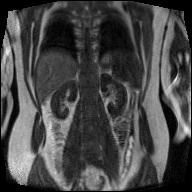
\includegraphics[height=0.26\linewidth]{img/preview/00}}\quad
		\subfloat[$t = 9\,Tp$]{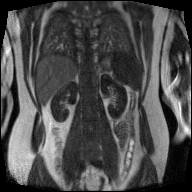
\includegraphics[height=0.26\linewidth]{img/preview/09}}\quad
			\subfloat[$t  = 12\,Tp$]{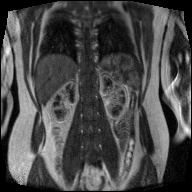
\includegraphics[height=0.26\linewidth]{img/preview/12}}\vspace{-4pt}
			
			
			\subfloat[$t  = 16\,Tp$]{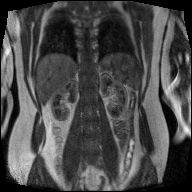
\includegraphics[height=0.26\linewidth]{img/preview/16}}	\quad		
			\subfloat[$t  = 18\,Tp$]{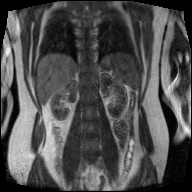
\includegraphics[height=0.26\linewidth]{img/preview/18}} \quad
		\subfloat[$t  = 22\,Tp$]	{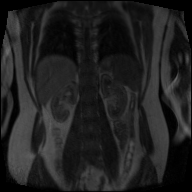
\includegraphics[height=0.26\linewidth]{img/preview/22}}\vspace{-4pt}
		
		
		\subfloat[$t  = 26\,Tp$]{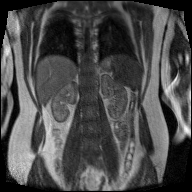
\includegraphics[height=0.26\linewidth]{img/preview/26}} \quad
			\subfloat[$t  = 30\,Tp$]{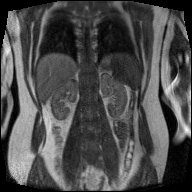
\includegraphics[height=0.26\linewidth]{img/preview/30}} \quad
			\subfloat[$t = 34\,Tp$]{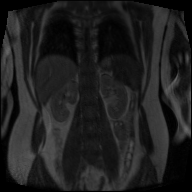
\includegraphics[height=0.26\linewidth]{img/preview/34}}\vspace{-4pt}
			
		\subfloat[$t  = 39\,Tp$]	{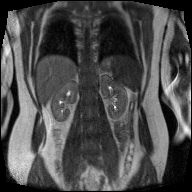
\includegraphics[height=0.26\linewidth]{img/preview/39}} \quad
	\subfloat[$t  = 55\,Tp$]{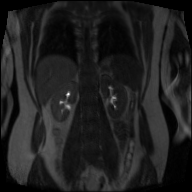
\includegraphics[height=0.26\linewidth]{img/preview/55}} \quad
	\subfloat[$t  = 73\, Tp$]{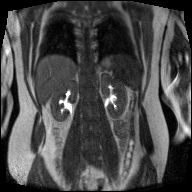
\includegraphics[height=0.26\linewidth]{img/preview/73}}
\vspace{0.2cm}
\caption[Sample DCE-MRI sequence of the healthy kidneys.]{Sample DCE-MRI sequence of the healthy kidneys. $Tp$ is a given time point. Firstly, the signal enhancement is observed in the renal cortex. Then, the tracer travels to the renal medulla and finally is collected by the collecting system}
\label{fig:set}
\end{figure}

\newpage
\section{GFR reference values}
Next to the DCE-MRI examinations, the participants had their GFR assessed by two chemical methods commonly used in the clinical practice: the \textit{serum-creatinine} (SCr) blood test and \textit{iohexol-GFR} tests. Creatinine is an endogenous indicator, which allows for estimating GFR from validated algorithms.
Iohexol in terms is an exogenous marker which is used for accurate GFR measurement. The clinical characteristics of all the participants are included in Table~\ref{tab:participants}

\begin{table}[h!]
\centering
\caption[Clinical characteristics of the participants]{Clinical characteristics of the participants \cite{eikefjord2017dynamic}}
\label{tab:participants}
\begin{threeparttable}
\rowcolors{2}{}{middleblue!30}
\renewcommand{\arraystretch}{1.25}
\begin{tabular}{L{7cm} R{4cm}}
	\toprule

 	Participants & 20\\
  	Gender (female/male) &16/4\\
  	Age (years) & 25 (20--38)\\
  	Height [m] & 1.71\,$\pm$\,0.07\\
  	Weight [kg] & 66.2\,$\pm$\,8.7\\
  	Body Mass Index (BMI) [kg/m\textsuperscript{2}] & 22.6\,$\pm$\,2.1\\
  	Body Surface Area (BSA) [m\textsuperscript{2}]& 1.77\,$\pm$\,0.14 (1.5--2.0) \\
  	Iohexol GFR [mL/min/m\textsuperscript{2}] &103\,$\pm$\,10 (87--125)\\
  	SCr GFR [mL/min/m\textsuperscript{2}] & 110\,$\pm$\,15 (81--128)\\
  \bottomrule

\end{tabular}
\begin{tablenotes}%
\footnotesize{}%
\item Values in parentheses are ranges.
\item Plus minus values are means $\pm$ standard deviations (SD).
    \end{tablenotes}
	\end{threeparttable}
\end{table}
\vspace{-0.1cm}
\section{Image processing and analysis}

\subsection{Motion correction}
One of the first fundamental problem encountered during DCE-MRI analysis is misalignment of the 3D volumes across time slices. This misalignment of organs is a result of the patient's respiratory motion as well as the heartbeat and bowel peristalsis and is unavoidable during examination. Studies have shown that even slight misalignment can lead to significant differences in intensity time courses \cite{KidneySubsegmentation} and thus, motion correction of time series is essential for further analysis.

In order to remove 	the motion artifact, all files were motion-corrected across time points. For this purpose the R programming language for statistical computing and graphics was used \cite{R} together with the package ANTsR \cite{ANTsR}, which provides quantification tools for biomedical images. 

As an initial step, for every time series, the algorithm extracts the 3D volumes. Each extracted volume corresponds to the data obtained in one time point. Next, the average image of the temporal volumes is calculated, which serves as a target image for image registration. Every temporal volume is then aligned to it and at the end they are combined back together into the 4D time series.
As the misalignment concerns the inner structures, not the whole body and various organs have spatially variant geometric differences, the modality of choice was the  \textit{symmetric normalisation} (SyN) algorithm, which is the non-rigid deformable transformation utilizing \textit{cross-correlation} (CC) as a similarity metric \cite{avants2011reproducible, avants2008symmetric, el2016current}. 

\subsection{Manual labelling}
In the next step, the labels of the whole left and right kidney were created. For this purpose the 3D volumes were extracted for each time frame and the slice with maximal signal enhancement of the kidneys was chosen (usually between 12--17 time slice). In this image, left and right kidney were manually delineated in coronal plane using the ITK-Snap software \cite{itk-snap}. Additionally, a few voxels of aorta (15--20) were labelled on maximal aortic enhancement time slice (9--10). So obtained labels were then combined and propagated across the time points. The sample labels are shown in Figure~\ref{fig:labels}.
All further analysis was implemented in the Python programming language~v.~3.6 \cite{python}.
\vspace{1cm}
\begin{figure}[H]
\captionsetup[subfloat]{captionskip=0.5cm}
	\centering
	\subfloat[Labels of the left and right kidneys]{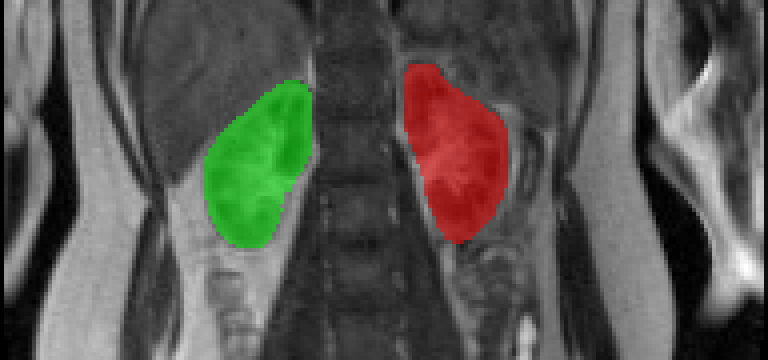
\includegraphics[width=0.48\textwidth ]{kidneys}}\hspace{0.02\textwidth}
	\subfloat[Label of the aorta]{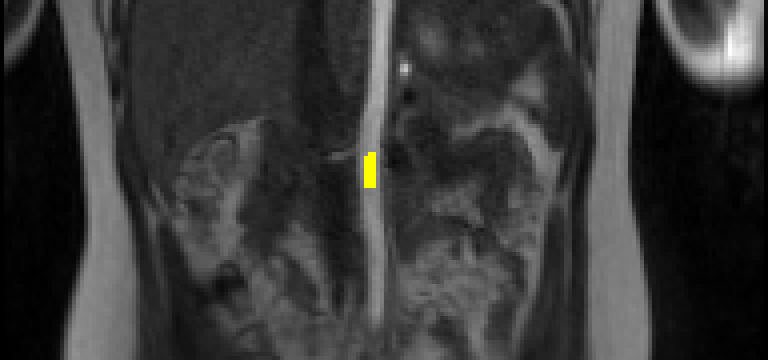
\includegraphics[width=0.48\textwidth]{aorta}}\\	
\vspace{0.5cm}
\caption[Sample labels of kidneys and aorta]{Sample labels of kidneys and aorta. Green and red are labels of the right and left kidney respectively, whereas yellow is the aorta label}
\label{fig:labels}
\end{figure}

\subsection{Pelvis region removal}
Due to the fact that glomerular filtration takes place in renal parenchyma, the region of pelvis had to be removed from further analysis. 

Resulting from the physiology of the process, the three renal compartments (cortex, medulla, pelvis) can be distinguished from each other on the basis of their time courses, as shown in Figure~\ref{fig:timecourses}. Depending on the compartment, the rapid enhancement of the signal occurs in different periods, which makes the shapes of the time intensity curves very unique.
From the Figure~\ref{fig:timecourses} it can be seen that the highest variation is observed between pelvis and two other renal compartments.
Consequently, it can be separated by unsupervised clustering.


\begin{figure}
	\centering
	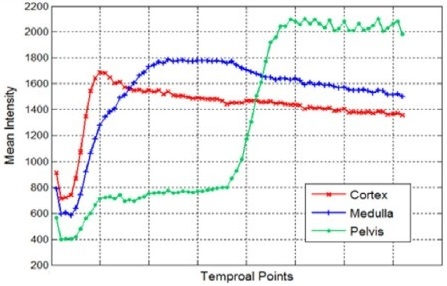
\includegraphics[width=10cm]{img/timecourses}
	\caption[Example kidney compartments time courses]{Example kidney compartments time courses \cite{KidneySubsegmentation}}
	\label{fig:timecourses}
\end{figure}


First of all, each voxel included in the label of the kidney was described by the vector of seventy-four features as follows:
\begin{equation}
\label{eq:voxel}
\mathbf{v_{ijk}} = [S(0),\; S(1),\;...\;,\; S(72),\; S(73)],
\end{equation}
where $S(n)$ is the value of signal intensity at the time point $n$.
\newpage

However, feature space of seventy-four dimensions is way too large for further analysis. High dimensionality of raw DCE-MRI data results in computational complexity, and thus memory and time consumption as well as numerical problems. What is more, it contains a lot of noise \cite{KidneySubsegmentation}. To overcome this problems, the \textit{principal component analysis} (PCA) \cite{pca} was applied.

PCA is a statistical procedure, which transforms the number of interrelated features into smaller set of uncorrelated variables. These so-called \textit{principal components} (PCs) are the linear combinations of the original variables \cite{dunteman1989principal}. As a result, after rotating the feature space, the first PC contains most variance, the last one the least and so on. In this way the dominant patterns are extracted, while the noise is reduced~\cite{pca, jolliffe1986principal}. Further, every of the PC is characterised by a ratio of \textit{explained variance}, which indicates the portion of the dataset’s variance lying along the axis of each PC~\cite{handson}.

Applying the theory to practice, each voxel belonging to the kidney, initially described by the seventy-four features was described by a number of PCs:
\begin{equation}
\label{eq:voxelpca}
\mathbf{v_{ijk}} = [PC1,\; PC2,\;...\;,\; PCn]  
\end{equation}
The amount of PCs, $n$, was chosen as a minimum number of dimensions required to preserve 95\% of the data's total variance so that the sum of the explained variances of  $n$ PCs was equal to at least 0.95 (usually between 4--6 PCs). The visual representation of the feature space with first three dimensions (PCs) for sample kidney is shown in Figure~\ref{fig:pca_plot}. Note that for better understanding, the clusters were already marked with different colors. 

\begin{figure}[H]
		\centering
		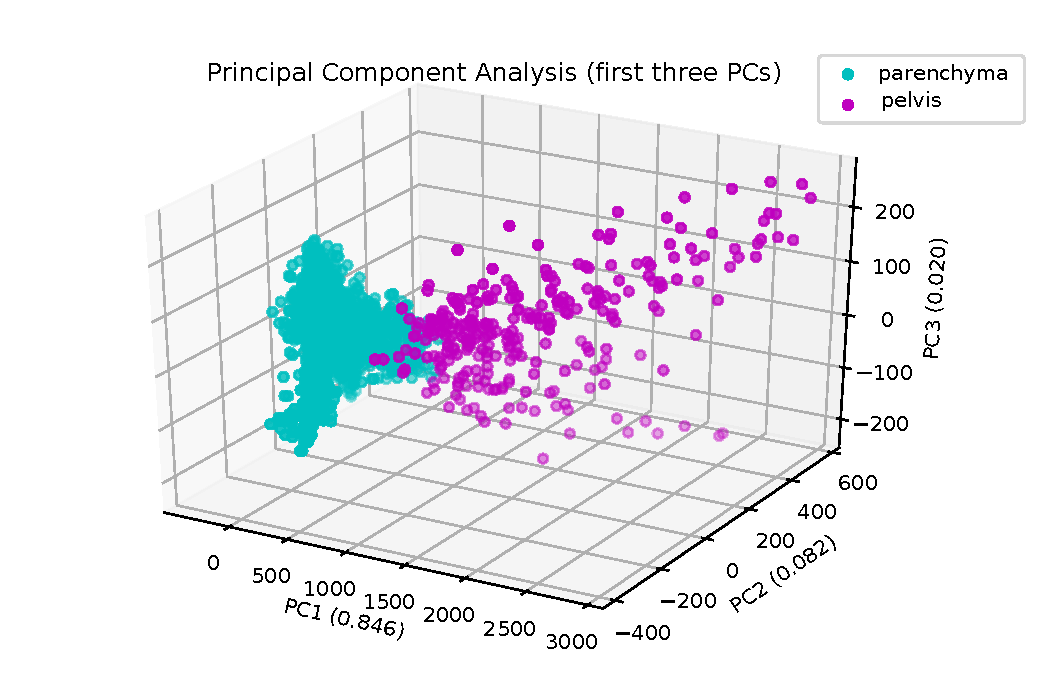
\includegraphics [height = 10cm]{pca3}
		\caption [Principal component analysis for a sample kidney]{Principal component analysis for a sample kidney. The values in brackets are the ratios of explained variance for the given PCs. Note that the number of PCs was reduced to three for visualisation purpose}
		\label{fig:pca_plot}
	\end{figure}

To the dimensionally reduced data, the \textit{k-means clustering}} was applied in order to separate voxels into two groups: pelvis and renal parenchyma. 
The k-means is an unsupervised clustering algorithm aiming to divide the data into groups so that the diversity between the groups and the similarity within the single group are maximised  \cite{kmeans}. 

Given a data set $X=\{ \vec{x_1}...\vec{x_n}$\} in $m$-dimensional space (which actually corresponds to the $m$ features of a sample) the algorithm's objective is to minimize the square error function given by  \cite{kmeans, alsabti1997efficient}:

\begin{equation}
	\label{eq:kmeans}
	J = \sum_{j=1}^{k}\sum_{x_i \in S_j}(||x_i-c_j||)^2,
\end{equation}
where $||x_i-c_j||$ is  the Euclidean distance between a data point $x_i$ and the cluster centre $c_j$ of cluster $S_j$ from $k$ predefined clusters. It is achieved in the steps summarised in Algorithm~\ref{alg:kmeans}.

\vspace{16pt}
\begin{algorithm}[H]
\footnotesize
    \SetKwInOut{Input}{Input}
    \SetKwInOut{Output}{Output}
    \SetKwFunction{RandomlyChooseCentroids}{RandomlyChooseCentroids}
    \SetKwFunction{CalculateMeanOfPointsInCluster}{CalculateMeanOfPointsInCluster}
    \SetKwData{Centroids}{$(\vec{c_1}...\vec{c_k})$}
    \SetKwFunction{argminDistance}{argminDistance}
    
	\Input{number of clusters $k$,\\ set of points in $m$-dimensional space: $X=\{ \vec{x_1}...\vec{x_n}$\}}
	
    \Output{set of cluster labels of $X$: $L = \{l(\vec{x_i})\;i \in\{1...n\}\}$ ,\\ coordinates of cluster centroids: \Centroids}
    
    \BlankLine
    \BlankLine
    
    
	\DontPrintSemicolon
	\Centroids $\leftarrow$ \RandomlyChooseCentroids{$k$, $X$} \Centroids$\in X$\;
    
	\Repeat{none of \Centroids changes}{
\tcc {assign each data point to the closest centroid on the basis of Euclidean distance}
$l(\vec{x_i})\leftarrow$\argminDistance($\vec{x_i}$, $\vec{c_j}$) $j \in\{1...k\}$ \\
\Centroids$\leftarrow$  \CalculateMeanOfPointsInCluster{}  \tcc*{recalculate centroids} 
}
	\Return{$L$ , \Centroids} \tcc*{points divided into clusters} 
    
    
    \SetAlgoCaptionSeparator{.}
    \caption{K-means clustering}
    \label{alg:kmeans}
\end{algorithm}

\vspace{16pt}
To segment the kidney, the k-means algorithm was initiated with two clusters, $k$~=~2 and performed for points (kidney voxels) in $m$-dimensional space ($m$ is the number of PCs).
Further, for each of the identified clusters, the average time point, $T_{max}$ in which signal intensity reaches its maximum was calculated. 
Following the assumption that $T_{max\_pelvis}>T_{max\_parenchyma}$, the cluster with greater $T_{max}$ was marked as the pelvis and removed from the ROI.
The average time-intensity curves for two detected clusters in k-means clustering algorithm for sample kidney are presented in Figure~\ref{fig:clusters}. One can easily note that the wash-in phase in pelvis takes place much later than in renal parenchyma. The results of the segmentation in turn are shown in Figure \ref{fig:segmentation}.  
\vspace{1cm}

\begin{figure}[H]
%\captionsetup[subfloat]{captionskip=0.5cm}
	\centering
	\includegraphics[width = \textwidth]{clusters}
	
\caption[Average time courses for two clusters detected in k-means algorithm]{Average time courses for two clusters detected in k-means algorithm performed for sample kidney}
\label{fig:clusters}
\end{figure}
\vspace{1cm}
\begin{figure}[H]
\captionsetup[subfloat]{captionskip=0.5cm}
	\centering
	\subfloat[Kidney segmentation]{\includegraphics[width=0.48\textwidth ]{kidney_pelvis}}\hspace{0.02\textwidth}
	\subfloat[Renal parenchyma]{\includegraphics[width=0.48\textwidth]{no_pelvis}}\\	
\vspace{0.5cm}
\caption[Sample kidney segmentation with k-means clustering]{The results of the segmentation obtained with k-means clustering. Figure (a) shows two regions of a sample kidney: the pelvis (magenta) and the renal parenchyma (cyan); Figure (b) presents the kidney after pelvis removal. The images were intentionally presented at Time point $t = 73\,Tp$, when the enhancement of the pelvis is high, for better visualisation}
\label{fig:segmentation}
\end{figure}

\newpage
\subsection{Concentration-time curves}
Having labelled the proper ROI, the time has come for the principal part of the analysis, namely pharmacokinetic modelling.
The whole PK part was implemented in the Python programming language from the scratch and no ready toolboxes for PK modelling were used.

All PK models used during quantitative DCE-MRI analysis call for determining both the tissue, $C_t(t)$, and blood plasma, $C_p(t)$, concentration as a~function of time. In our case, the $C_t(t)$ is the mean concentration in renal parenchyma, whereas the
$C_p(t)$, can be derived from the AIF, which is a concentration in a blood vessel feeding the kidney (aorta).
Thus, they were calculated in the next steps of the project.  

For each of the kidney, as well as for the aorta, the mean intensities of the voxels included in the particular labels were calculated at the each time point and the intensity time courses were plotted. Sample time courses are shown in Figure~\ref{fig:temporal_points}.

\vspace{50pt}
\begin{figure}[H]
%\captionsetup[subfloat]{captionskip=0.5cm}
	\centering
	\includegraphics[width = \textwidth]{temporal_points}
	
\caption[Sample average time-intensity curves for a kidney and aorta with marked last points of the baseline]{Sample average time-intensity curves for a kidney and aorta. Red dot is $T_{baseline}$, the last point of the baseline}
\label{fig:temporal_points}
\end{figure}



\newpage
Assuming the linear relation between tracer concentration and signal intensity $S(t)$ dictated by the low dose of Ga-based CA, the tracer concentration can be expressed as:
\begin{equation}
	\label{eq:conversion}
	C(t) = S(t)-S_0,
\end{equation}
where $S_0$ is the baseline signal, which is the average signal intensity among the time before the administration of CA. 
In order to determine $S_0$, the time point before rapid signal increase, $T_{baseline}$ had to be found  as marked with red dot in Figure \ref{fig:temporal_points}.

To achieve it, firstly, for the purposes of the examination of the function changes, the median filter  with the $kernel\;size = 5$ was applied in order to smooth the signal and eliminate artificial  peaks and valleys, as shown in Figure~\ref{fig:median}  
In next step, for every intensity time course under analysis, its derivative was calculated. The derivative describes the instantaneous rate of change of the function. It tells how fast the output of the function (signal intensity) changes compared to the independent variable (time) \cite{calculus} and seems to be a perfect solution to the problem, which boils down to finding the most rapid signal change. 
Because of one's interests is detection only of the function's increases, not decreases, the points, in which the derivative is negative were neglected, $S'(t)<0\leftarrow0$. So modified derivative of the sample kidney and aorta are shown in Figure~\ref{fig:derivative}.

Now, all that had to be done to find $T_{baseline}$ was to detect the point, in which the derivative of the signal intensity time course reaches its maximum, $T_{baseline}=argmax\;S'(t)$. Having it determined, the $S_0$ was calculated as the mean signal intensity value from the beginning of the measurement ($t=0$) to $T_{baseline}$. Finally, the CA concentration in the tissue and aorta were calculated according to Formula~(\ref{eq:conversion}). The results of intensity-concentration conversion for sample time curves are shown in Figure~\ref{fig:conversion}.
\newpage 
\vspace*{0cm}
\begin{figure}[H]
%\captionsetup[subfloat]{captionskip=0.5cm}
	\centering
	\includegraphics[width = \textwidth]{median2}
\caption[Sample average time-intensity curves for a kidney and aorta with applied median filter]{Sample average time-intensity curves for a kidney and aorta with applied median filter. Note that cut peak of the aorta's signal is a result of the median filter and it is present only during the baseline removal step}
\label{fig:median}
\end{figure}

\begin{figure}[H]
%\captionsetup[subfloat]{captionskip=0.5cm}
	\centering
	\includegraphics[width = \textwidth]{derivative}
\caption[Positive derivative of the sample kidney and aorta intensity time courses]{Positive derivative of a sample kidney and aorta intensity time courses. The vertical line indicates the time point, in which the derivative reaches its maximal value}
\label{fig:derivative}
\end{figure}

\begin{figure}[H]
%\captionsetup[subfloat]{captionskip=0.5cm}
	\centering
	\includegraphics[width = \textwidth]{conversion}
\caption[Time courses of a sample kidney and aorta after intensity-concentration conversion]{Time-intensity curves of a sample kidney and aorta converted into the concentration-time curves}
\label{fig:conversion}
\end{figure}


\subsection{Pharmacokinetic modelling}

Having determined the AIF and the concentration time course for the renal pa\-ren\-chy\-ma, almost all components necessary for the renal quantitative evaluation were obtained. Almost, but not all. One should take into consideration the fact that AIF is the concentration of CA in the blood of the aorta, which consist of both the red blood cells and the blood plasma. Gadolinium-based contrast agents, however, distribute in plasma rather than whole blood, so their effective plasma concentrations must be considered. Thus, the \textit{hematocrit} (Hct) correction was performed as follows \cite{tofts2010t1}:
\begin{equation}
	\label{eq:hematocrit}
	C_{p}(t) = \frac{C_{a}(t)} {1-Hct},
\end{equation}
where $C_p$ is CA plasma concentration, $C_a$ is concentration in the aorta defined by the AIF and $Hct$ is the fractional volume of red blood cells in the blood. In this study, its value was taken from the literature as an average population value and was equal to $Hct=0.42$ \cite{tofts2010t1}.

Finally, PK modelling could have been performed. The models of choice were the Tofts and Kermode model, extended Tofts and Kermode model, Patlak-Rutland model and two-compartment exchange model. The aim was to obtain value of the transfer constant $K_{trans}$ [min$^-1$], which corresponds to the GFR per unit tissue volume. The fit was performed by using a non-linear least squares analysis.
 
\paragraph{Tofts and Kermode model.}
According to the \textit{Tofts and Kermode} (TK) model \cite{tofts1991measurement} the tracer is distributed in two compartments: intravascular and \textit{extravascular extra-cellular space} (EES).
The tracer diffuses from the blood plasma at rate specified by the transfer constant $K_{trans}$ [min$^{-1}$] and returns at the reverse transfer rate $k_{ep} = K_{trans}/v_e$ [min$^{-1}$]. This model assumes, however, that the amount of intravascular (plasma) tracer is negligible comparing to the tissue signal. 
The tissue concentration, $C_t(t)$, is then given by \cite{khalifa2014models}:
\begin{equation}
C_t(t) = v_eC_e(t),
\end{equation}
\noindent where $v_e$ is EES fractional volume and $C_e(t)$ is EES concentration. The system can be described by mass balance equation  \cite{khalifa2014models, tofts1999estimating}: 
\begin{equation}
	\label{eq:toft}
	\frac{dC_{t}(t)}{dt} = K_{trans}(C_p(t)-C_t(t)/v_e),
\end{equation} 
where  and $C_p(t)$ is blood plasma concentration, The solution obtained according to the procedure presented in Chapter~\ref{chapter:pk} is \cite{sourbron2011scope, khalifa2014models}:
\begin{equation}
	\label{eq:toft2}
	C_{t}(t) =C_p\circledast K_{trans}e^{-k_{ep}t} =K_{trans}\int_{0}^{t}C_p(\tau)e^{-k_{ep}(t-\tau)}d\tau  
\end{equation}
\newpage
\paragraph{Extended Tofts and Kermode model.}
While the Tofts model neglects intravascular contribution assuming weak vascularization of the tissue, the \textit{extended Tofts and Kermode} (ETK) model \cite{tofts1997modeling} does take it into account. According to ETK, the tissue concentration is described by the formula \cite{tofts2010t1, khalifa2014models}:
\begin{equation}
C_t(t) = v_pC_p(t) + v_eC_e(t),
\label{eq:etk}
\end{equation}
where $v_p$ is fractional plasma volume. The differential equation describing the EES compartment is \cite{sourbron2011scope}:
\begin{equation}
	\label{eq:etoft}
	v_e\frac{dC_{e}(t)}{dt} = K_{trans}(C_p(t)-C_e(t))
\end{equation}
Solving the equation and substituting to (\ref{eq:etk}) the tissue concentration boils down to \cite{khalifa2014models, tofts2010t1}:
\begin{align}
	\label{eq:extended_toft}
	C_{t}(t) &=v_pC_p(t) + C_p\circledast K_{trans}e^{-k_{ep}t} =\\
	\nonumber &= v_pC_p(t)+K_{trans}\int_{0}^{t}C_p(\tau)e^{-k_{ep}(t-\tau)}d\tau 
\end{align}


In TK and ETK models the free parameters $K_{trans}$, $v_e$ and $v_p$ are estimated by fitting the model to obtained in DCE-MRI examinations time-concentration curves.  
\paragraph{Patlak-Rutland model.}
Unlike the TK and ETK models, the \textit{Patlak-Rutland} model \cite{patlak1983graphical} assumes that reverse transfer constant from the EES to the plasma, $k_{ep}$, is negligibly small, because of the short time of the measurement (tracer does not have time to return) and low permeability \cite{khalifa2014models}. 
Similarly to the ETK, the tissue concentration is equal to:
\begin{equation}
C_t(t) = v_pC_p(t) + v_eC_e(t)
\label{eq:patlak1}
\end{equation}
\newpage
\noindent However, the tracer change in EES is equal to \cite{thesis,patlak1983graphical}: 
\begin{equation}
	\label{eq:patlak2}
	v_e\frac{dC_{e}(t)}{dt} = K_{trans}C_p(t)
\end{equation}
Solving the Equation (\ref{eq:patlak2}) and substituting into Formula (\ref{eq:patlak2}) \cite{khalifa2014models, patlak1983graphical}: 
\begin{equation}
	\label{eq:patlak}
	C_{t}(t) =v_pC_p(t) + K_{trans}\int_{0}^{t}C_p(\tau)d\tau  
\end{equation}
To obtain the free parameters, the concentration time courses obtained from DCE-MRI examination can be fitted directly to Formula (\ref{eq:patlak}) or the graphical approach called the \textit{Patlak plot} can be applied. In this approach the above equation is linearised as \cite{khalifa2014models, patlak1983graphical}:  
\begin{equation}
	\label{eq:patlak_lin}
	Y = K_{trans}X +v_p,  
\end{equation}
where $Y=C_t(t)/C_p(t)$ and $X=\int_{0}^{t}C_p(\tau)d\tau/C_p(t)$. The free parameters $K_{trans}$ and $v_p$ can be then estimating by constructing a linear plot and calculating its slope and intercept respectively.
In this project, the data was fitted to Formula (\ref{eq:patlak}). 

\paragraph{Two-compartment exchange model.}While all the previously described models allow for estimating transfer constant $K_{trans}$ combining both the plasma blood flow, and the tissue permeability, \textit{two-compartment exchange model} (2CXM) enables their separate estimation. 
According to 2CXM, the plasma compartment has an arterial inlet and a venous outlet of the same plasma flow, $Fp$ [min$^{-1}$]. 
The tracer is exchanged between the two compartments: EES and intravascular plasma, at a~symmetric rate quantified by the permeability surface product, $PS$ [min$^{-1}$].
Because the CA leaves the system, the model is referred to as an open system. 
Similarly to PR and ETK models the tissue concentration is expressed as \cite{khalifa2014models}:
\begin{equation}
C_t(t) = v_pC_p(t) + v_eC_e(t)
\label{eq:2cxm}
\end{equation}
The system is described by a pair of mass balance differential equations \cite{khalifa2014models}:  
\begin{equation}
v_p\frac{dC_p(t)}{dt} = F_p(C_a(t)-C_p(t))+PS(C_e(t)-C_p(t))
\label{eq:2cxm2}
\end{equation}
\begin{equation}
v_e\frac{dC_e(t)}{dt} = PS(C_p(t)-C_e(t))
\label{eq:2cxm3}
\end{equation}
Note that in 2CXM the CA concentration in the plasma of the feeding artery is denoted as $C_a$ ($C_p$ in previous models) whereas $C_p$ is CA concentration in intravascular plasma. The solution boils down to \cite{khalifa2014models}:
\begin{align}
	\label{eq:2cxm4}
	\nonumber C_{t}(t) &=F_p (Be^{-m_1t}+(1-B)e^{-m_2t})\circledast C_a =\\
	&= F_{p} \int_{0}^{t} \left( Be^{-m_1\tau} + (1-B)e^{-m_2\tau} \right) C_{a}(t-\tau)d\tau,
\end{align}
where $m_1$, $m_2$ and $B$ are defined as:
\begin {equation} 
m_1 = \frac{1}{2}\left( a+b+\sqrt{(a+b)^2-4bc}\right)
\end{equation}
\begin {equation} 
\nonumber m_2 = \frac{1}{2}\left(a+b-\sqrt{(a+b)^2-4bc}\right)
\end{equation}
\begin {equation} 
\nonumber B = \frac{m_2-c}{m_2-m_1}, 
\end{equation}
where
\begin{equation}
a = \frac{F_p+PS}{v_p},\qquad b = \frac{PS}{v_e},\qquad c = \frac{F_p}{v_p}
\end{equation}
The $K_{trans}$ can be then obtained by:
\begin{equation}
K_{trans} = \frac{PS\cdot{}F_p}{PS+F_p}
\end{equation}

A sample concentration time course fitted to different models is shown in Figure~\ref{fig:fit}. 

\begin{figure}
\captionsetup[subfloat]{captionskip=0.5cm}
	\centering
	\subfloat[TK model fit; $K_{trans}$ = 0.52 min$^{-1}$ ]{\includegraphics [width=0.48\linewidth]{tk2}}\hspace{0.03\linewidth}
	\subfloat[ETK model fit; $K_{trans}$ = 0.45 min$^{-1}$]{\includegraphics[width=0.48\linewidth]{etk2}}\\ \vspace{1cm}	
	\subfloat[PR model fit; $K_{trans}$ = 0.19 min$^{-1}$]{\includegraphics [width=0.48\linewidth]{pr2}}\hspace{0.03\linewidth}
	\subfloat[2CXM model fit; $K_{trans}$ = 0.37 min$^{-1}$]{\includegraphics[width=0.48\linewidth]{2cxm2}}\\	
\vspace{1cm}
\caption[An example of models fit]{A sample concentration time course fitted to different PK models: (a) Tofts and Kermode model (b) extended Tofts and Kermode model (c) Patlak-Rutland model (d) two-compartment exchange model}
\label{fig:fit}
\end{figure}

\subsection{GFR estimation}
Having estimated the transfer constant $K_{trans}$ the \textit{Single Kidney GFR} (SKGFR) could have been calculated according to the formula:
\begin{equation}
SKGFR = K_{trans}V_{parenchyma},
\end{equation}
where $V_{parenchyma}$ is the parenchymal volume (in mL) of the examined kidney given by:
\begin{equation}
V_{parenchyma} = nV_{voxel},
\end{equation}
where $n$ is the number of voxels included in the kidney label whereas $V_{voxel}$ is the volume of the voxel (2.2\,$\times$\,2.2\,$\times$\,3\,mm$^3$ = 0.14252 mL). Total GFR for each dataset was then calculated by summing up the SKGFR of the left and right kidneys. All obtained GFR values were normalised for standard BSA (1.73\,m$^2$).


%----------------------------------------------------------------------------------------
%	Section: Results
%----------------------------------------------------------------------------------------

\newpage
%\section{Results}
%\label{sec:Results}
%The segmentation of the pelvis was evaluated with Dice similarity coefficient given by the formula:
\begin{equation}
	\label{eq:dice}
	DS = \dfrac{2|A}{•},
\end{equation}
where $||x_i-c_j||$ is  the Euclidean distance between a data point $x_i$ and the cluster centre $c_j$ of k predefined clusters. 
The segmentation of the pelvis obtained for the sample kidney is shown on the Figure \ref{fig:kidney_segmented}. 

The example of the time concentration curves after baseline removal for the kidney and aorta are shown on Figure \ref{fig:removed_baseline}. 

Fitting of the time course for different pharmacokinetic models  is illustreted on the Figure~\ref{fig:models}.



\begin{figure*}[h!]
	\centering
	\subfloat[Segmented kidney]{\includegraphics[height=4 cm]{img/kidney_pelvis}}\quad
	\subfloat[Parenchymal volume]{\includegraphics[height=4 cm]{img/no_pelvis}}\\	
	\caption{The sample segmented kidney (a) and parenchymal volume with removed pelvis (b) purple - renal parenchyma, blue - renal pelvis.}
\label{fig:kidney_segmented}
\end{figure*}


\begin{figure*}[h!]
	\centering
	\subfloat[Kidney time course]{\includegraphics[width=7 cm]{img/kidney_no_baseline}}\quad
	\subfloat[Aorta time course]{\includegraphics[width=7 cm]{img/aorta_no_baseline}}\\	
\caption{Sample average time-concentration curves for renal parenchyma (a) and aorta (b). The red curve shows the original data while the blue one - after baseline removal.}
\label{fig:removed_baseline}
\end{figure*}

\begin{figure*}[h!]
	\centering
	\subfloat[Toft's model]{\includegraphics[width=4.5 cm]{img/tk}}\quad
	\subfloat[Extended Toft's model]{\includegraphics[width=4.5 cm]{img/etk}}\quad
	\subfloat[Patlak model]{\includegraphics[width=4.5 cm]{img/patlak}}\\	
\caption{Fit of the time-concentration curve of sample kidney to three different PK models.}
\label{fig:models}
\end{figure*}

\newpage



%----------------------------------------------------------------------------------------
%	Section: Conclusions
%----------------------------------------------------------------------------------------

\newpage
%\section{Conclusions}
%\label{sec:Conclusions}
%\input{./tex/conclusions}

%----------------------------------------------------------------------------------------
%	Section: Summary
%----------------------------------------------------------------------------------------

\newpage
%\section{Summary}
%\label{sec:Summary}
%\chapter{Summary}

%\addcontentsline{toc}{chapter}{Summary}

The main purposes of this thesis were, firstly, to design a library in Python programming language for pharmacokinetic modelling from DCE-MRI images, which is to be incorporated into the fast method of GFR estimation, and secondly, to compare the performance of the few PK models for application of assessing renal function and to examine whether any of them can be considered accurate and precise enough to be used in the target method.

As a first step, the DCE-MRI sequences were registered in a time domain and both kidneys as well as aorta were manually labelled. Next, the renal pelvis was removed from the kidneys' labels on the basis of voxels' intensity time courses. For this purpose the PCA together with k-means clustering was applied. Subsequently, the average time-intensity curves were obtained for both kidneys and aorta. The signal intensity was converted into concentration by finding the temporal point, at which positive $S'(t)$ reaches the maximum value. So obtained concentration time courses were then fitted to four pharmacokinetic models: Tofts Kermode, Extended Tofts Kermode, Rutland Patlak and two-compartment exchange models. Finally, on the basis of the obtained parameters the SKGFR as well as total GFR were calculated and compared with two chemical methods. 
  
The developed algorithm was tested on the DCE-MRI sequences of ten different participants. Dice similarity coefficient of the pelvis segmentation was equal to DSC~=~0.86\,$\pm$\,0.06. For each of the sequence the pelvis was removed correctly without the need of manual correction. Regarding the performance of different PK models, the obtained results show that 2CXM is the most accurate and precise one and gives results comparable with those of the SCr blood test, which is a commonly used clinical method. What is more, the obtained $P30 = 100\%$ for this model proves that its estimation is sufficient to be used in clinical use.   

All in all, the thesis was a success. An important contribution is creating the module in Python, which will be used in further research on fast method of GFR estimation.  
On the basis of the drawn conclusions of practical tests the 2CXM model can be applied as a final step of the target method.

The source code is available at \underline{\url{https://github.com/KasiaSprawka}}.


%----------------------------------------------------------------------------------------
%	REFERENCE LIST
%----------------------------------------------------------------------------------------
%\newpage
%\addcontentsline{toc}{section}{References}
%\bibliographystyle{ieeetr}
%\bibliography{./tex/references}\\


%----------------------------------------------------------------------------------------
%	APPENDICES
%----------------------------------------------------------------------------------------

%\newpage
%\section*{Appendices}
%\addcontentsline{toc}{section}{Appendices}
%\label{sec:Appendices}
%\subsection*{\textbf{Appendix A:} The abstract accepted for ECR (the European Congress of Radiology)}

\begin{center}

\includegraphics[trim={0 3.5cm 0 1cm},clip,height = 19 cm]{appendices/abstract}

\end{center}

\newpage
\subsection*{\textbf{Appendix B:} The code implemented for pharmacokinetic modelling}

Under cleaning


\end{document}
